% ===========================================================================
% ANN MPI 并行化实验报告
% ===========================================================================
\documentclass[a4paper,11pt,UTF8]{ctexart}

\usepackage{fontspec}
\usepackage[a4paper,left=2.4cm,right=2.4cm,top=2.55cm,bottom=2.55cm]{geometry}
\usepackage{amsmath}
\usepackage{amssymb}
\usepackage{booktabs}
\usepackage{caption}
\usepackage{enumitem}
\usepackage{float}
\usepackage{graphicx}
\usepackage[pdfpagelabels=false,pageanchor=false]{hyperref}
\usepackage{listings}
\usepackage{fancyhdr}
\usepackage{xcolor}
\usepackage{array}
\usepackage{tabularx}
\usepackage{multirow}
\usepackage{tikz}
\usetikzlibrary{positioning,arrows.meta,fit,calc}

\graphicspath{{./}{fig/}}
\hypersetup{colorlinks=true,linkcolor=black,urlcolor=black,citecolor=black}
\linespread{1.12}
\renewcommand{\contentsname}{目录}
\renewcommand{\figurename}{图}
\renewcommand{\tablename}{表}
\setcounter{tocdepth}{1}
\setlength{\parindent}{2em}
\setlength{\parskip}{2pt}
\setlength{\textfloatsep}{11pt plus 2pt minus 2pt}
\setlength{\intextsep}{9pt plus 2pt minus 2pt}
\setlength{\abovecaptionskip}{5pt}
\setlength{\belowcaptionskip}{3pt}
\setlength{\abovedisplayskip}{7pt}
\setlength{\belowdisplayskip}{7pt}
\setlength{\emergencystretch}{2.5em}
\captionsetup{font=small,labelsep=quad}
\setlist{leftmargin=1.8em,itemsep=2pt,topsep=3pt}

\newcommand{\code}[1]{\texttt{\detokenize{#1}}}
\newcommand{\fcell}[2]{\begin{tabular}[t]{@{}l@{}}\code{#1}\\\code{#2}\end{tabular}}
\newcommand{\HRule}{\rule{\linewidth}{0.45mm}}
\newcolumntype{Y}{>{\raggedright\arraybackslash}X}
\newcolumntype{C}[1]{>{\centering\arraybackslash}p{#1}}

\lstset{
  basicstyle=\ttfamily\footnotesize,
  keywordstyle=\color{blue!70!black},
  commentstyle=\color{green!40!black},
  numbers=left,
  numberstyle=\tiny,
  frame=single,
  breaklines=true,
  columns=fullflexible,
  aboveskip=5pt,
  belowskip=5pt,
  mathescape=false
}

\pagestyle{fancy}
\fancyhf{}
\lhead{\kaishu ANN 近似最近邻搜索}
\rhead{\kaishu 并行程序设计实验报告}
\cfoot{}
\setlength{\headheight}{14pt}
\renewcommand{\headrulewidth}{0.1pt}
\fancypagestyle{tocstyle}{
  \fancyhf{}
  \lhead{\kaishu 目录}
  \rhead{\kaishu 并行程序设计实验报告}
  \cfoot{\thepage}
  \renewcommand{\headrulewidth}{0.1pt}
  \renewcommand{\footrulewidth}{0pt}
}
\renewcommand{\today}{2026 年 6 月 6 日}

\begin{document}

\pagestyle{empty}

\begin{titlepage}
  \begin{center}
    
\includegraphics[width=0.78\textwidth]{NKU.png}\\[1cm]
    \vspace{18mm}
    {\huge\kaishu 计算机学院\par}
    \vspace{0.5cm}
    {\huge\kaishu 并行程序设计实验报告\par}
    \vspace{1.9cm}
    {\Huge\kaishu MPI 编程实验\par}
    \vspace{0.35cm}
    {\Huge\kaishu ANN 近似最近邻搜索\par}
    \vspace{0.55cm}
    {\Large\kaishu 从算法原理到分布式架构的设计剖析\par}
    \vspace{0.25cm}
    {\Large\kaishu IVF-PQ / Block-HNSW / IVF-HNSW / HNSW-on-HNSW\par}

    \vspace{\fill}
    {\LARGE\kaishu 姓名：柯云超\par}
    \vspace{0.45cm}
    {\LARGE\kaishu 学号：2413575\par}
    \vspace{0.45cm}
    {\LARGE\kaishu 专业：计算机科学与技术\par}
    \vspace{0.45cm}
    {\Large\kaishu 代码仓库：\href{https://github.com/kyc001/parallel}{github.com/kyc001/parallel}\par}

    \vfill
    {\Large \today\par}
  \end{center}
\end{titlepage}

\clearpage
\begingroup
\pagestyle{tocstyle}
\thispagestyle{tocstyle}
\tableofcontents
\endgroup

\clearpage
\pagenumbering{arabic}
\renewcommand{\thefigure}{\thesection{}.\arabic{figure}}
\renewcommand{\thetable}{\thesection{}.\arabic{table}}
\makeatletter
\@addtoreset{figure}{section}
\@addtoreset{table}{section}
\makeatother
\pagestyle{fancy}
\cfoot{正文 \thepage\ /\ \pageref{LastBodyPage}}

\section*{摘要}
\addcontentsline{toc}{section}{摘要}

近似最近邻搜索迁移到 MPI 后，首要问题变成：哪些工作留在 rank 本地完成，哪些信息必须跨 rank 交换，才能在保持全局 top-$k$ 正确性的同时控制通信量和负载尾部。实现上，MPI 层被压缩成一个轻量候选协议：rank 0 负责数据分发、query 广播、候选收集和全局合并；每个 rank 独立维护本地 IVF-PQ 或 HNSW 系列索引，并在 rank 内用 OpenMP 生成本地候选。索引实现只需返回固定长度候选数组，MPI 层不介入索引内部搜索。

正文从 ANN 的 top-$k$ 定义和 MPI 通信边界出发，依次讨论 owner-computes 数据划分、候选协议、critical path 计时和 rank 本地自治四个约束；随后用架构图和伪代码说明 base shard、query broadcast、本地搜索、候选 gather 和 rank 0 merge 的完整路径；再比较 IVF-PQ、Block-HNSW、IVF+HNSW 与 HNSW-on-HNSW 四类局部候选生成器的原理与取舍。实验部分只保留验证设计假设所需的关键结果，复现命令、文件清单、实验矩阵和 AI 使用记录统一放入附录。

DEEP100K 双平台实验表明：相同参数下 Windows MS-MPI 与鲲鹏 PBS 的 Recall 完全一致，全局 id 映射和分布式 top-$k$ merge 逻辑稳定；在 \code{np=8, threads=2, query=2000} 的代表配置中，通信与 merge 占比约为 1\% 量级，表 \ref{tab:comm_ratio} 中最高为 1.20\%，主要瓶颈仍在 rank 内 ANN 搜索。相对 SIMD 实验中的原始串行 Flat，本次 Windows 侧 MPI IVF-PQ 最优点达到 $19.67\times$ 的累计加速，鲲鹏侧达到 $51.76\times$；Block-HNSW 在两平台的对照还显示，MPI 迁移既可能是低延迟加速，也可能是高召回和分布式候选合并能力的取舍。HNSW-on-HNSW 证明了分层图索引可行，但全 block 探测需要用更高延迟换取接近满召回。VTune 与硬件事件进一步指出，距离内核已经走 AVX SIMD 路径，高召回图索引的限制主要来自不规则图遍历、候选队列维护、TLB/DRAM 压力和负载尾部。

\noindent\textbf{关键词：} ANN；MPI；OpenMP；IVF-PQ；HNSW；HNSW-on-HNSW；负载均衡；通信开销

\section{问题描述与实验目标}

\subsection{问题切入：分布式搜索不是把循环拆开}

给定基向量集合
\[
X=\{x_0,x_1,\ldots,x_{N-1}\}, \quad x_i\in \mathbb{R}^{96},
\]
以及 query 向量 $q$，ANN 搜索返回与 $q$ 最接近的 $k$ 个候选。本实验沿用前两次 ANN 作业的内积距离：
\[
d(x,q)=1-\sum_{j=0}^{d-1}x_jq_j.
\]
Recall@$k$ 定义为返回集合与 ground truth top-$k$ 的交集比例：
\[
\mathrm{Recall@}k=\frac{|KNN(q)\cap KANN(q)|}{k}.
\]

如果只在单进程中并行，ANN 的主要问题是如何更快地产生候选；迁移到 MPI 后，问题变成了“多个局部候选集合能否组合成一个正确的全局结果”。简单地把 base 平均切给多个进程并不自动成立，因为它会引入三类新约束：
\begin{enumerate}
  \item \textbf{正确性约束：}每个 rank 只知道自己的 shard，局部 top-$k$ 必须携带原始全局 id，rank 0 才能和 ground truth 对齐；
  \item \textbf{通信约束：}不能把局部原始向量或大候选池传回 root，否则 MPI 层会吞掉 shard 缩小带来的收益；
  \item \textbf{尾部约束：}一次分布式查询要等最慢 rank 结束，本地搜索时间的最大值比平均值更能决定端到端延迟。
\end{enumerate}

因此，实验的重点不在于把一个 for 循环机械拆成 $P$ 段，而在于为 ANN 搜索建立可组合的分布式协议：每个 rank 负责拥有的数据，跨 rank 只交换足够恢复全局 top-$k$ 的最小候选信息。

\subsection{设计原则}

实现按四条约束展开。

\begin{enumerate}
  \item \textbf{Owner-computes：}base shard 分给谁，就由谁构建索引并完成本地搜索。在线阶段不跨 rank 访问远端索引，避免把 HNSW 的随机访问扩展成网络通信。
  \item \textbf{固定长度候选协议：}每个 rank 对每个 query 只返回 $k$ 个 \code{(distance, global_id)}，rank 0 从 $P\times k$ 个候选中恢复全局 top-$k$。通信量随 $QPk$ 增长，不随 base 数据量增长。
  \item \textbf{关键路径计时：}总延迟拆为 $\max_i T_i^{search}+T^{comm+merge}$。以最慢 rank 作为本地搜索项，可以把负载不均衡与通信开销区分开。
  \item \textbf{局部候选生成器抽象：}IVF-PQ、Block-HNSW、IVF+HNSW 与 HNSW-on-HNSW 都实现为本地索引和本地 top-$k$ 生成器；MPI 外壳不关心索引内部结构，只负责候选协议。
\end{enumerate}

\subsection{报告结构}

报告正文只保留理解设计和判断取舍所需的内容。复现脚本、结果文件、实验矩阵和 AI 使用记录放在附录，避免正文被命令和日志路径打断。

\begin{table}[H]
  \centering\footnotesize
  \begin{tabularx}{\textwidth}{p{3.2cm}Yp{2.5cm}}
    \toprule
    关注点 & 设计问题 & 对应章节 \\
    \midrule
    总体架构 & MPI 层、OpenMP 层和索引层如何分工。 & 第 3 节 \\
    合并正确性 & 局部 top-$k$ 为什么足以恢复全局 top-$k$。 & 第 3 节 \\
    索引设计 & 四种候选生成器分别牺牲什么、换来什么。 & 第 3 节 \\
    实验设计 & 用哪些指标验证通信、负载和召回假设。 & 第 2 节 \\
    参数与扩展性 & 设计旋钮如何改变候选空间和 rank 粒度。 & 第 4 节 \\
    瓶颈定位 & 通信、负载尾部和 rank 内图遍历哪个更重要。 & 第 4、5 节 \\
    复现细节 & 命令、文件、实验矩阵和 AI 使用说明。 & 附录 \\
    \bottomrule
  \end{tabularx}
  \caption{正文阅读线索：从设计问题到验证证据}
  \label{tab:reading_map}
\end{table}

\section{实验平台、数据集与测量方法}

\subsection{平台与数据集}

实验使用 DEEP100K 数据集：base 向量 $N=100000$，维度 $d=96$，query 和 ground truth 使用课程提供的二进制文件。正式实验统一取前 \code{query_n=2000} 条 query，$k=10$。平台信息见表 \ref{tab:env}。正文只讨论 Windows MS-MPI 与鲲鹏 PBS 两个平台，因为它们分别覆盖了本地真实 MPI 开发环境和课程服务器提交环境。

\begin{table}[H]
  \centering\small
  \begin{tabularx}{\textwidth}{p{3.1cm}p{3.6cm}Y}
    \toprule
    平台 & MPI/编译环境 & 用途 \\
    \midrule
    Windows 本地 & MS-MPI，MinGW-w64，AVX2/FMA 参数 &
    本地开发、真实 MPI 参数扫描、扩展性、混合布局、亲和性实验，以及 rank-local VTune 剖析。\\
    鲲鹏 PBS & AArch64 Linux，服务器 MPI 编译器，PBS 队列，\code{/anndata} 共享数据 &
    按提交指南验证作业提交路径，完成同样的参数扫描、扩展性实验和通信模式实验。\\
    \bottomrule
  \end{tabularx}
  \caption{实验平台与用途。报告正文只展示 Windows MS-MPI 与鲲鹏 PBS 两个平台结果。}
  \label{tab:env}
\end{table}

\subsection{测量目标与验证假设}

前文的架构设计可以转化为四个可验证假设。
\begin{enumerate}
  \item \textbf{合并协议不引入正确性损失。}如果全局 id 映射和候选布局正确，相同参数在不同平台上应得到一致 Recall。
  \item \textbf{通信不是当前主瓶颈。}如果固定长度候选协议有效，\code{comm+merge latency} 应远小于本地搜索时间。
  \item \textbf{进程数存在拐点。}增加 MPI rank 会缩小每个 shard，但也会增加固定通信、同步、调度和负载尾部；因此 \code{np=8} 不一定优于 \code{np=4}。
  \item \textbf{高召回图索引受 rank 内局部性限制。}若 HNSW 类方法的瓶颈来自图遍历而非 MPI，VTune 应看到候选队列、随机访存、TLB/DRAM 和后端停顿，而不是单纯的通信等待。
\end{enumerate}

\subsection{评价指标与计时口径}

程序为所有模式输出统一字段：
\begin{itemize}
  \item \code{average recall}：Recall@10；
  \item \code{average latency (us)}：从 query broadcast 到 rank 0 merge 完成的平均单 query 时间；
  \item \code{max local search latency (us)}：所有 rank 中最慢本地搜索时间；
  \item \code{comm+merge latency (us)}：总在线时间减去最慢本地搜索时间，近似表示广播、gather、reduce 和 merge 的合计开销；
  \item \code{per-rank search latency (us)}：每个 rank 的本地搜索时间，用于计算负载不均衡度。
\end{itemize}

\code{comm+merge latency} 用总在线时间减去最慢 rank 本地搜索时间得到，没有把各个 MPI API 的局部计时简单相加。这个口径更贴近分布式查询的关键路径：如果某个 rank 更慢，rank 0 必须等待它，等待时间属于负载尾部，不应计入通信协议本身。所有正文图表都来自保存的日志和解析 CSV；完整脚本、文件清单和实验矩阵见附录 \ref{sec:appendix_repro} 至附录 \ref{sec:appendix_matrix}。

\section{算法设计与实现}

\subsection{分层架构}

架构上先把“分布式协调”和“近邻候选生成”分开。MPI 层只处理所有算法都相同的边界问题：数据切分、query 分发、候选回收和全局合并；OpenMP 层只在 rank 内部工作；索引层则可以替换为 IVF-PQ、Block-HNSW、IVF+HNSW 或 HNSW-on-HNSW。这个边界带来的直接效果是：新增局部 ANN 索引时，不需要重新设计通信协议；实验阻塞/非阻塞 gather 或 MPI 线程级别时，也不需要改动索引原理。

\begin{figure}[H]
  \centering
  \resizebox{0.96\textwidth}{!}{%
  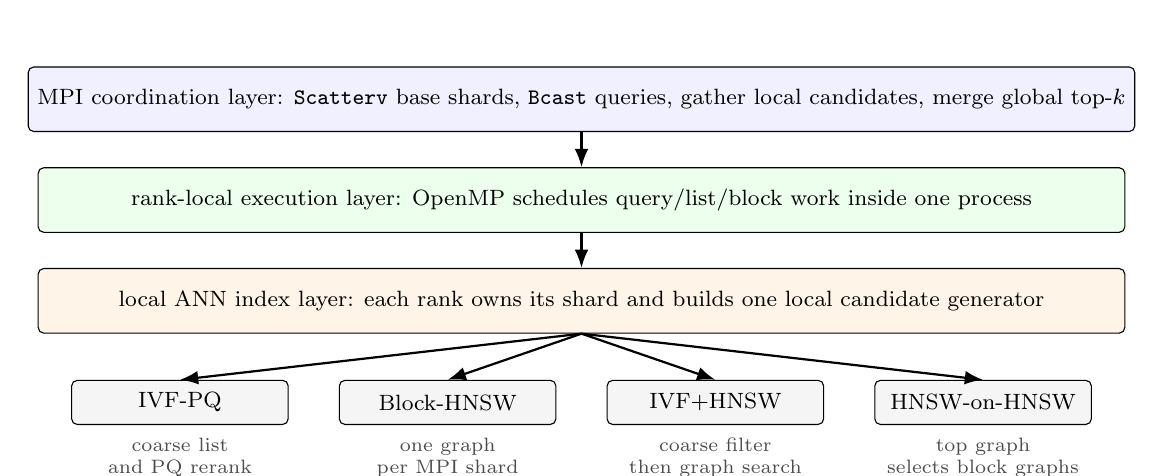
\begin{tikzpicture}[
    font=\footnotesize,
    layer/.style={draw,rounded corners=2pt,minimum width=13.8cm,minimum height=0.82cm,align=center},
    cell/.style={draw,rounded corners=2pt,minimum width=2.75cm,minimum height=0.56cm,align=center},
    arr/.style={-Latex,thick},
    note/.style={font=\scriptsize,align=center,text=black!70}
  ]
    \node[layer,fill=blue!6] (mpi) at (0,2.0) {MPI coordination layer: \code{Scatterv} base shards, \code{Bcast} queries, gather local candidates, merge global top-$k$};
    \node[layer,fill=green!7] (omp) at (0,0.72) {rank-local execution layer: OpenMP schedules query/list/block work inside one process};
    \node[layer,fill=orange!9] (idx) at (0,-0.56) {local ANN index layer: each rank owns its shard and builds one local candidate generator};

    \node[cell,fill=gray!8] (ivfpq) at (-5.1,-1.85) {IVF-PQ};
    \node[cell,fill=gray!8] (block) at (-1.7,-1.85) {Block-HNSW};
    \node[cell,fill=gray!8] (ivfh) at (1.7,-1.85) {IVF+HNSW};
    \node[cell,fill=gray!8] (hoh) at (5.1,-1.85) {HNSW-on-HNSW};

    \draw[arr] (idx.south) -- (block.north);
    \draw[arr] (idx.south) -- (ivfpq.north);
    \draw[arr] (idx.south) -- (ivfh.north);
    \draw[arr] (idx.south) -- (hoh.north);
    \draw[arr] (mpi.south) -- (omp.north);
    \draw[arr] (omp.south) -- (idx.north);

    \node[note] at (-5.1,-2.55) {coarse list\\and PQ rerank};
    \node[note] at (-1.7,-2.55) {one graph\\per MPI shard};
    \node[note] at (1.7,-2.55) {coarse filter\\then graph search};
    \node[note] at (5.1,-2.55) {top graph\\selects block graphs};
  \end{tikzpicture}
  }
  \caption{分层架构：MPI 只规定候选协议，索引层作为可替换的本地候选生成器。}
  \label{fig:layered_arch}
\end{figure}

\subsection{MPI 数据流}

整体结构如图 \ref{fig:mpi_flow} 所示。rank 0 负责读取 DEEP100K 的 base/query/ground truth 文件，然后通过 \code{MPI_Scatterv} 将 base 向量按连续区间分给所有 rank。每个 rank 只在自己的 \code{local_base} 上构建本地索引。在线查询阶段，rank 0 将 query 批量 \code{MPI_Bcast} 到所有进程；每个进程独立搜索本地 shard，打包本地 top-$k$ 候选，再通过 gather 汇总到 rank 0；最后 rank 0 对所有候选做全局 top-$k$ merge，并计算 Recall@10。

\begin{figure}[H]
  \centering
  \resizebox{\textwidth}{!}{%
  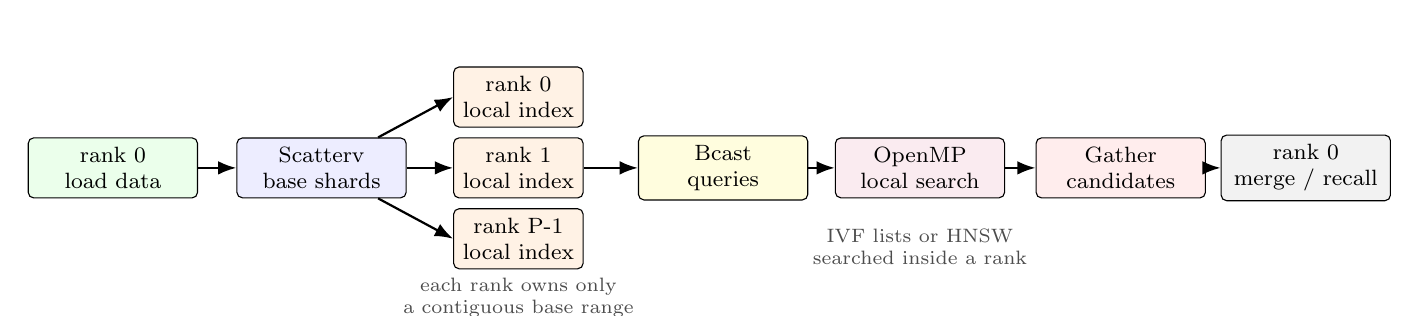
\begin{tikzpicture}[
    font=\footnotesize,
    stage/.style={draw,rounded corners=2pt,align=center,minimum width=2.15cm,minimum height=0.66cm},
    rank/.style={draw,rounded corners=2pt,align=center,minimum width=1.45cm,minimum height=0.52cm,fill=orange!10},
    arr/.style={-Latex,thick},
    hint/.style={align=center,font=\scriptsize,text=black!70}
  ]
    \node[stage,fill=green!8] (data) at (0,1.1) {rank 0\\load data};
    \node[stage,fill=blue!7] (scatter) at (2.65,1.1) {Scatterv\\base shards};
    \node[rank] (r0) at (5.15,2.0) {rank 0\\local index};
    \node[rank] (r1) at (5.15,1.1) {rank 1\\local index};
    \node[rank] (rp) at (5.15,0.2) {rank P-1\\local index};
    \node[stage,fill=yellow!13] (bcast) at (7.75,1.1) {Bcast\\queries};
    \node[stage,fill=purple!8] (search) at (10.25,1.1) {OpenMP\\local search};
    \node[stage,fill=red!7] (gather) at (12.8,1.1) {Gather\\candidates};
    \node[stage,fill=gray!10] (merge) at (15.15,1.1) {rank 0\\merge / recall};

    \draw[arr] (data) -- (scatter);
    \draw[arr] (scatter) -- (r0.west);
    \draw[arr] (scatter) -- (r1.west);
    \draw[arr] (scatter) -- (rp.west);
    \draw[arr] (r1.east) -- (bcast);
    \draw[arr] (bcast) -- (search);
    \draw[arr] (search) -- (gather);
    \draw[arr] (gather) -- (merge);

    \node[hint] at (5.15,-0.55) {each rank owns only\\a contiguous base range};
    \node[hint] at (10.25,0.1) {IVF lists or HNSW\\searched inside a rank};
  \end{tikzpicture}
  }
  \caption{MPI + OpenMP 混合 ANN 搜索流程。MPI 负责跨进程数据分发和结果归并，OpenMP 只作用于每个 rank 的本地搜索。}
  \label{fig:mpi_flow}
\end{figure}

\subsection{负载划分}

代码中使用 \code{PartitionRange(n, rank, world_size)} 对 base 向量做连续分块。设进程数为 $P$，则每个 rank 得到
\[
\left\lfloor \frac{N}{P}\right\rfloor
\quad\text{或}\quad
\left\lceil \frac{N}{P}\right\rceil
\]
个向量，最大只差 1。连续划分的优点是实现简单、传输时可直接使用 \code{MPI_Scatterv} 的 displacement，同时每个 rank 的 \code{local_base} 连续存储，有利于本地 cache locality。缺点是如果数据分布本身有明显偏斜，某些 rank 的搜索路径可能更长；因此程序额外打印 \code{per-rank search latency (us)}，并用
\[
\mathrm{imbalance}=\frac{\max_i T_i}{\frac{1}{P}\sum_i T_i}
\]
衡量最慢 rank 与平均 rank 的差异。

分布式 cache locality 主要体现在两层。第一，\code{MPI_Scatterv} 后每个 rank 的 base shard 是一段连续 \code{float} 数组，IVF-PQ 的 reordered list、PQ 编码和 HNSW 构图都只访问本进程内存，避免跨 rank 的远程随机访存；候选 gather 只传输 compact 的 top-$k$ 结果，而不是把原始向量拉回 rank 0。第二，默认连续切分保留了原始 id 的空间局部性，候选 id 映射代价很低；启用随机打散时，程序同步 scatter 一份 \code{local_global_ids}，以很小的额外整数数组代价保留全局 id 正确性。连续切分的代价是随机化不足：如果原始 base 顺序本身带有类别或聚类偏斜，某些 rank 可能持有更难搜索的局部图。后文的 imbalance 指标正是用来判断这种 locality 与负载均衡之间的取舍。

\begin{lstlisting}[language=C++]
Range PartitionRange(size_t n, int rank, int world_size) {
    const size_t base = n / world_size;
    const size_t extra = n % world_size;
    const size_t begin = rank * base + std::min<size_t>(rank, extra);
    const size_t count = base + (rank < extra ? 1 : 0);
    return {begin, begin + count};
}
\end{lstlisting}

\subsection{局部搜索与全局合并}

每个 rank 的局部搜索结果以 top-$k$ 堆形式保存。为了跨进程传输，程序将每个 query 的 top-$k$ 打包成两个定长数组：距离 \code{float} 和全局 id \code{uint64_t}。rank 0 收到所有 rank 的候选后，对每个 query 扫描 $P\times k$ 个候选并维护全局 top-$k$ 堆。因此 merge 的复杂度近似为
\[
O(QPk\log k),
\]
其中 $Q$ 是 query 数。与本地搜索的 IVF 或 HNSW 访问相比，当 $P$ 和 $k$ 不大时，这部分开销很小。正式全量实验中 $P=8,k=10,Q=2000$，每个 rank 发送约 $Qk(4+8)\approx 234$ KiB 候选数据，query 广播约 $Qd\cdot4\approx 750$ KiB，因此通信量仍小于本地索引搜索的访存量。

局部 top-$k$ 足以恢复全局 top-$k$ 的原因也很直接。对任意 query，假设某个向量 $x$ 属于全局 top-$k$，但它没有出现在所属 rank 的局部 top-$k$ 中，那么同一 rank 内至少存在 $k$ 个向量比 $x$ 更近；这些向量当然也属于全局候选空间，于是全局范围内已经至少有 $k$ 个向量优于 $x$，这与 $x$ 属于全局 top-$k$ 矛盾。因此，只要每个 rank 返回精确的局部 top-$k$，rank 0 扫描所有局部 top-$k$ 就不会漏掉真正的全局 top-$k$。近似性只来自各 rank 内的 ANN 索引本身，而不来自 MPI 合并协议。

候选缓冲区按“query 优先、rank 次之、候选序号最后”的顺序组织。这样做的原因是 rank 0 在合并时天然按 query 扫描，内层只需要从每个 rank 取出该 query 的 $k$ 个局部候选，不必重新解析变长消息。图 \ref{fig:candidate_merge} 给出了这一布局和合并过程。

\begin{figure}[H]
  \centering
  \resizebox{0.95\textwidth}{!}{%
  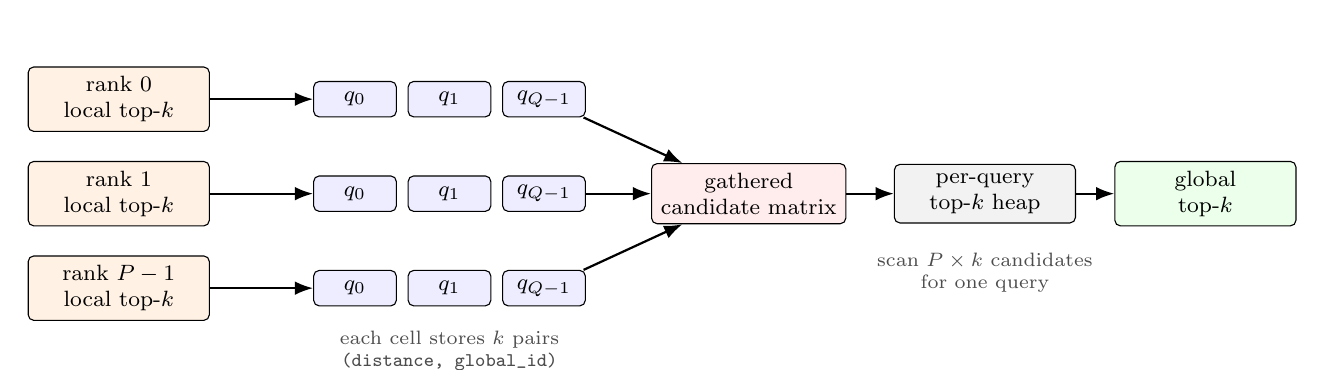
\begin{tikzpicture}[
    font=\footnotesize,
    box/.style={draw,rounded corners=2pt,align=center,minimum width=2.3cm,minimum height=0.55cm},
    smallbox/.style={draw,rounded corners=2pt,align=center,minimum width=1.05cm,minimum height=0.45cm},
    arr/.style={-Latex,thick},
    note/.style={font=\scriptsize,align=center,text=black!70}
  ]
    \node[box,fill=orange!10] (r0) at (0,1.2) {rank 0\\local top-$k$};
    \node[box,fill=orange!10] (r1) at (0,0) {rank 1\\local top-$k$};
    \node[box,fill=orange!10] (rp) at (0,-1.2) {rank $P-1$\\local top-$k$};

    \node[smallbox,fill=blue!7] (q0a) at (3.0,1.2) {$q_0$};
    \node[smallbox,fill=blue!7] (q1a) at (4.2,1.2) {$q_1$};
    \node[smallbox,fill=blue!7] (qna) at (5.4,1.2) {$q_{Q-1}$};
    \node[smallbox,fill=blue!7] (q0b) at (3.0,0) {$q_0$};
    \node[smallbox,fill=blue!7] (q1b) at (4.2,0) {$q_1$};
    \node[smallbox,fill=blue!7] (qnb) at (5.4,0) {$q_{Q-1}$};
    \node[smallbox,fill=blue!7] (q0c) at (3.0,-1.2) {$q_0$};
    \node[smallbox,fill=blue!7] (q1c) at (4.2,-1.2) {$q_1$};
    \node[smallbox,fill=blue!7] (qnc) at (5.4,-1.2) {$q_{Q-1}$};

    \node[box,fill=red!7] (gather) at (8.0,0) {gathered\\candidate matrix};
    \node[box,fill=gray!10] (heap) at (11.0,0) {per-query\\top-$k$ heap};
    \node[box,fill=green!8] (out) at (13.8,0) {global\\top-$k$};

    \draw[arr] (r0) -- (q0a);
    \draw[arr] (r1) -- (q0b);
    \draw[arr] (rp) -- (q0c);
    \draw[arr] (qna) -- (gather);
    \draw[arr] (qnb) -- (gather);
    \draw[arr] (qnc) -- (gather);
    \draw[arr] (gather) -- (heap);
    \draw[arr] (heap) -- (out);

    \node[note] at (4.2,-2.0) {each cell stores $k$ pairs\\\code{(distance, global_id)}};
    \node[note] at (11.0,-1.0) {scan $P\times k$ candidates\\for one query};
  \end{tikzpicture}
  }
  \caption{rank 0 的候选矩阵与 top-$k$ 合并过程。每个 rank 只发送本地 top-$k$，最终输出仍按全局 id 计算 Recall。}
  \label{fig:candidate_merge}
\end{figure}

合并逻辑对应的伪代码如下。代码中距离越小代表越接近，因此堆顶保存当前全局 top-$k$ 中最差的候选；新候选更好时替换堆顶。

\begin{lstlisting}[language=C++]
for q in 0 .. query_n-1:
    heap = empty max_heap_by_distance()
    for r in 0 .. world_size-1:
        for j in 0 .. k-1:
            cand = gathered[r][q][j]
            if cand.id is invalid:
                continue
            if heap.size() < k:
                heap.push(cand)
            else if cand.distance < heap.top().distance:
                heap.pop()
                heap.push(cand)
    output[q] = sort_by_distance(heap)
\end{lstlisting}

\subsection{架构边界}

到这里可以把在线路径抽象成一个很小的接口：本地索引只需要实现“给定 query 批，返回每个 query 的本地 top-$k$”；MPI 外壳只需要知道这些候选的距离和全局 id。这个边界把复杂度限制在两个方向：
\begin{itemize}
  \item 索引内部可以很复杂，例如 IVF 粗筛、PQ rerank、HNSW 图遍历、分层 block 选择，但它们都不改变跨 rank 候选协议；
  \item MPI 通信可以切换为阻塞、非阻塞或不同线程级别，但它们都不改变本地 ANN 索引的数学含义。
\end{itemize}
工程目录、数据路径和复现脚本属于交付细节，统一放在附录 \ref{sec:appendix_engineering} 和附录 \ref{sec:appendix_repro} 中。正文后续只讨论这些边界为什么合理，以及实验结果是否支持这些设计选择。

\subsection{局部索引设计与并行边界}

\subsubsection{四种搜索模式}

本次实现不只保留一个 baseline，而是把 IVF 与图索引分支放进同一套 MPI 外壳中。它们在 MPI 层暴露同一个抽象接口：

\begin{lstlisting}[language=C++]
LocalIndex index = BuildLocalIndex(local_base, params, mode);
LocalTopK local = SearchLocal(index, queries, threads);
PackedCandidates msg = Pack(local, local_global_ids);
\end{lstlisting}

因此，四种算法的差异不在“如何通信”，而在“一个 rank 如何从自己的 shard 里产生足够好的局部候选”。表 \ref{tab:modes} 按设计取舍比较这些模式；具体命令行形式和复现入口移到附录。

\begin{table}[H]
  \centering\small
  \begin{tabularx}{\textwidth}{p{2.7cm}Y Y Y}
    \toprule
    模式 & 设计直觉 & rank 内并行边界 & 主要风险 \\
    \midrule
    IVF-PQ &
    先用粗聚类减少候选空间，再用 PQ 距离和 rerank 控制延迟。 &
    query/list 级并行；倒排表扫描较规则，适合批量 query。 &
    \code{nprobe} 太小会漏掉真实近邻所在区域，召回上限受粗筛限制。\\
    Block-HNSW &
    MPI shard 本身就是天然 block，每个 rank 建一张局部图。 &
    多 query 或多入口并行；单条图搜索路径内部依赖较强。 &
    图遍历不规则，rank 间 shard 难度不同会形成尾部。\\
    IVF+HNSW &
    用 IVF 先选局部簇，再在簇内用 HNSW 提高候选质量。 &
    簇间和 query 间可并行；簇内仍是图搜索。 &
    同时继承 IVF 漏筛和 HNSW 随机访问两类问题。\\
    HNSW-on-HNSW &
    先在 block 质心图上选 block，再搜索被选中的 bottom graph。 &
    被选 block 之间可并行，bottom graph 内部为局部图搜索。 &
    若为保证召回而探测全部 block，会退化为昂贵的多图搜索。\\
    \bottomrule
  \end{tabularx}
  \caption{统一 MPI 外壳下的四种本地候选生成器}
  \label{tab:modes}
\end{table}

\subsubsection{IVF-PQ 的 MPI 迁移}

IVF-PQ 是从上一阶段多线程版本迁移到 MPI 的基础方案。多线程版本中，一个进程维护完整索引；MPI 版本中，每个 rank 只维护本地 shard 的 inverted lists。query 被广播到所有进程后，各 rank 只在本地 list 中搜索，返回局部 top-$k$。由于每个 rank 只看到一部分 base data，最终的 top-$k$ 必须由 rank 0 对所有局部结果进行全局合并。

进程内仍复用 OpenMP inter-query 并行：当 query 批量足够大时，不同线程处理不同 query，写入不同结果槽，几乎不需要同步。这一点延续了前一次 Pthread/OpenMP 实验中“inter-query 粒度更稳健”的结论。

\subsubsection{图索引 A/B/C}

图索引部分实现了三种结构，分别对应“先筛选再图搜索”“分 rank 图搜索”和“分层图搜索”，结构如图 \ref{fig:graph_modes}。

\begin{figure}[H]
  \centering
  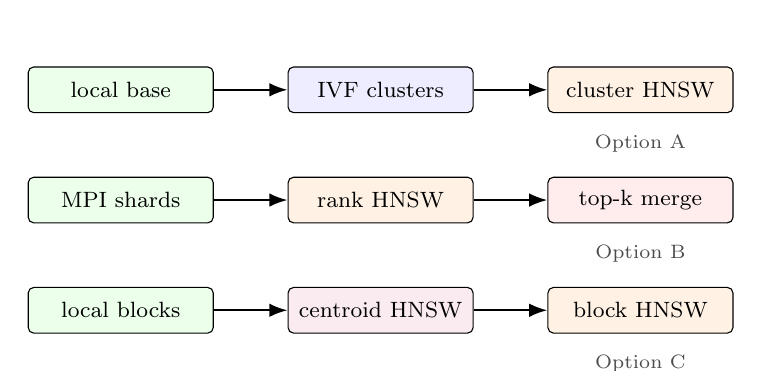
\begin{tikzpicture}[
    font=\footnotesize,
    box/.style={draw,rounded corners=2pt,align=center,minimum width=2.35cm,minimum height=0.58cm},
    arr/.style={-Latex,thick},
    note/.style={font=\scriptsize,align=center,text=black!70}
  ]
    \node[box,fill=green!8] (baseA) at (0,1.4) {local base};
    \node[box,fill=blue!7] (ivfA) at (3.3,1.4) {IVF clusters};
    \node[box,fill=orange!10] (hnswA) at (6.6,1.4) {cluster HNSW};
    \node[note] at (6.6,0.72) {Option A};
    \draw[arr] (baseA) -- (ivfA);
    \draw[arr] (ivfA) -- (hnswA);

    \node[box,fill=green!8] (baseB) at (0,0) {MPI shards};
    \node[box,fill=orange!10] (hnswB) at (3.3,0) {rank HNSW};
    \node[box,fill=red!7] (mergeB) at (6.6,0) {top-k merge};
    \node[note] at (6.6,-0.68) {Option B};
    \draw[arr] (baseB) -- (hnswB);
    \draw[arr] (hnswB) -- (mergeB);

    \node[box,fill=green!8] (baseC) at (0,-1.4) {local blocks};
    \node[box,fill=purple!8] (topC) at (3.3,-1.4) {centroid HNSW};
    \node[box,fill=orange!10] (blockC) at (6.6,-1.4) {block HNSW};
    \node[note] at (6.6,-2.08) {Option C};
    \draw[arr] (baseC) -- (topC);
    \draw[arr] (topC) -- (blockC);
  \end{tikzpicture}
  \caption{三类图索引方案：IVF+HNSW、分块 HNSW 和 HNSW-on-HNSW。}
  \label{fig:graph_modes}
\end{figure}

\textbf{方案 A：IVF+HNSW。}每个 rank 内先建立 IVF 粗聚类，随后在每个簇中单独建立 HNSW。搜索阶段先按 query 与质心距离选择 \code{nprobe} 个簇，再在这些簇的 HNSW 内搜索。它的优点是能避免搜索所有局部向量；缺点是召回依赖簇选择，若 ground truth 所在簇未被探测，则后续 HNSW 再精确也无法恢复。

\textbf{方案 B：分块 HNSW。}MPI 本身已经把 base 划分成多个 shard，因此每个 rank 的 HNSW 可以视为一个独立 block graph。所有 rank 并行搜索自己的图，rank 0 再合并结果。该方案实现直接、召回较高，但每个局部 HNSW 的搜索路径具有串行依赖，OpenMP 只能在多入口或多 query 层面分摊，不能把单条贪心路径线性拆开。

\textbf{方案 C：HNSW-on-HNSW。}分层图方案中，每个 rank 把本地 base 分成多个 block，先计算 block centroid 并建立 top-level HNSW；每个 block 内再建立 bottom-level HNSW。搜索时先在 centroid graph 上选择若干 block，再并行搜索被选中的 block graph。它能表达“图上再建图”的组合策略；当 \code{nprobe_blocks} 取满 16 时，全量实验 Recall@10 达到 0.99995，但因为实际搜索了所有 block，延迟明显上升。

\subsubsection{混合并行边界}

混合并行的关键不只是同时打开 MPI 和 OpenMP，而是明确划分职责：
\begin{itemize}
  \item MPI 层：base shard 分配、query 广播、候选 gather、最慢 rank 计时归约、rank 0 top-$k$ merge；
  \item OpenMP 层：rank 内 query/list/block 级并行，避免跨进程共享状态；
  \item 索引层：每个 rank 独立构建本地 IVF-PQ 或 HNSW，不在在线阶段跨进程访问远端索引。
\end{itemize}

这种边界使程序比较容易在 Windows MS-MPI 和鲲鹏 PBS 环境中复现。它也限制了通信复杂度：在线阶段只有一次 query broadcast 和一次候选 gather，没有在 HNSW 搜索路径中进行细粒度跨 rank 通信。

\subsubsection{在线阶段伪代码}

为了说明 MPI 代码的控制流，下面给出一次批量查询的伪代码。索引构建发生在计时前；报告中的 online latency 从 query broadcast 前的 barrier 之后开始计时，直到 rank 0 完成 merge 和 recall 计算前结束。

\begin{lstlisting}[language=C++]
range = PartitionRange(base_n, rank, world_size);
MPI_Scatterv(root_base, counts, displs, MPI_FLOAT, local_base);
index = BuildLocalIndex(local_base, mode);

MPI_Barrier(MPI_COMM_WORLD);
phase_begin = MPI_Wtime();
MPI_Bcast(queries, query_n * dim, MPI_FLOAT, 0, MPI_COMM_WORLD);

search_begin = MPI_Wtime();
local_topk = SearchLocal(index, queries, nthreads);
search_us = MPI_Wtime() - search_begin;

PackCandidates(local_topk, local_global_ids, local_distances, local_ids);
GatherCandidates(local_distances, local_ids, all_distances, all_ids);
MPI_Reduce(search_us, max_search_us, MPI_MAX, 0, MPI_COMM_WORLD);

if (rank == 0) {
    merged = MergeGatheredCandidates(all_distances, all_ids);
    total_us = MPI_Wtime() - phase_begin;
    comm_merge_us = total_us - max_search_us;
    recall = RecallAtK(merged, ground_truth);
}
\end{lstlisting}

这里使用 \code{MPI_Reduce} 的 \code{MPI_MAX} 而不是平均值，是因为一次分布式查询必须等最慢 rank 完成本地搜索后才能合并。因此总延迟应与最慢 rank 的搜索时间对齐，\code{comm+merge latency} 才能表示“除了最慢本地搜索以外的剩余开销”。如果用平均搜索时间，会把负载不均衡误计入通信开销。

\section{实验结果与分析}

\subsection{参数扫描：设计旋钮如何改变候选空间}

四种索引的参数本质上都在调节“每个 rank 为一个 query 打开多大的候选空间”。IVF-PQ 和 IVF+HNSW 用 \code{nprobe} 决定探测多少粗簇；Block-HNSW 用 \code{ef} 控制图搜索保留多少前沿候选；HNSW-on-HNSW 用 \code{nprobe_blocks} 决定进入多少底层 block graph。参数扫描的目的不是单纯找一组最快数字，而是观察候选空间扩大后，Recall 是否值得为增加的局部搜索代价买单。

\subsubsection{代表性参数点}

表 \ref{tab:default_points} 汇总了两平台在相同代表参数下的结果。所有点均来自参数扫描日志，统一使用 \code{np=8}、\code{threads=2}、\code{query_n=2000}。代表参数如下：
\begin{itemize}
  \item IVF-PQ：\code{nlist=16}、\code{nprobe=4}、\code{p=1000}；
  \item Block-HNSW：\code{ef=50}；
  \item IVF+HNSW：\code{nprobe=4}、\code{ef=50}；
  \item HNSW-on-HNSW：\code{nblocks=16}、\code{nprobe_blocks=16}、\code{ef=50}。
\end{itemize}

\begin{table}[H]
  \centering\footnotesize\setlength{\tabcolsep}{3.2pt}
  \begin{tabular}{p{2.8cm}p{2.9cm}C{1.4cm}C{1.7cm}C{1.7cm}C{1.7cm}C{1.5cm}}
    \toprule
    平台 & 算法 & Recall & latency & local max & comm & imbalance \\
    \midrule
    Windows MS-MPI & IVF-PQ & 0.96515 & 334.59555 & 331.10550 & 3.49005 & 1.06707 \\
    Windows MS-MPI & Block-HNSW & 1.00000 & 221.45235 & 218.78595 & 2.66640 & 1.00663 \\
    Windows MS-MPI & IVF+HNSW & 0.96450 & 326.40570 & 322.79650 & 3.60920 & 1.00457 \\
    Windows MS-MPI & HNSW-on-HNSW & 0.99995 & 2053.35915 & 2045.68515 & 7.67400 & 1.01303 \\
    \midrule
    鲲鹏 PBS & IVF-PQ & 0.96515 & 512.09760 & 509.37176 & 2.72584 & 1.04614 \\
    鲲鹏 PBS & Block-HNSW & 1.00000 & 765.25044 & 762.63249 & 2.61796 & 1.19441 \\
    鲲鹏 PBS & IVF+HNSW & 0.96450 & 911.40282 & 908.41758 & 2.98524 & 1.03207 \\
    鲲鹏 PBS & HNSW-on-HNSW & 0.99995 & 2489.16447 & 2486.21905 & 2.94542 & 1.17062 \\
    \bottomrule
  \end{tabular}
  \caption{双平台代表参数点。所有延迟单位均为 $\mu$s/query。}
  \label{tab:default_points}
\end{table}

相同算法参数下，两平台 Recall 完全一致，表明 base shard 的全局 id 偏移、候选 gather 顺序和 rank 0 top-$k$ merge 在跨平台上是稳定的。延迟上，Windows 的图索引明显更快；鲲鹏 PBS 的通信/merge 绝对值更低，但本地 HNSW 图搜索耗时更高，主要差异来自图访问、优先队列和分支路径，而不是 MPI 传输。

\subsubsection{Windows 参数曲线}

图 \ref{fig:param_windows} 给出 Windows MS-MPI 上的参数曲线。IVF-PQ 和 IVF+HNSW 的横轴随 \code{nprobe} 增大整体右移，同时 Recall 上升；Block-HNSW 随 \code{ef} 增大召回更稳定，但图搜索扩展邻居更多；HNSW-on-HNSW 的 \code{nprobe_blocks} 越大，越接近搜索全部 block，召回接近 1.0 时延迟迅速增加。

\begin{figure}[H]
  \centering
  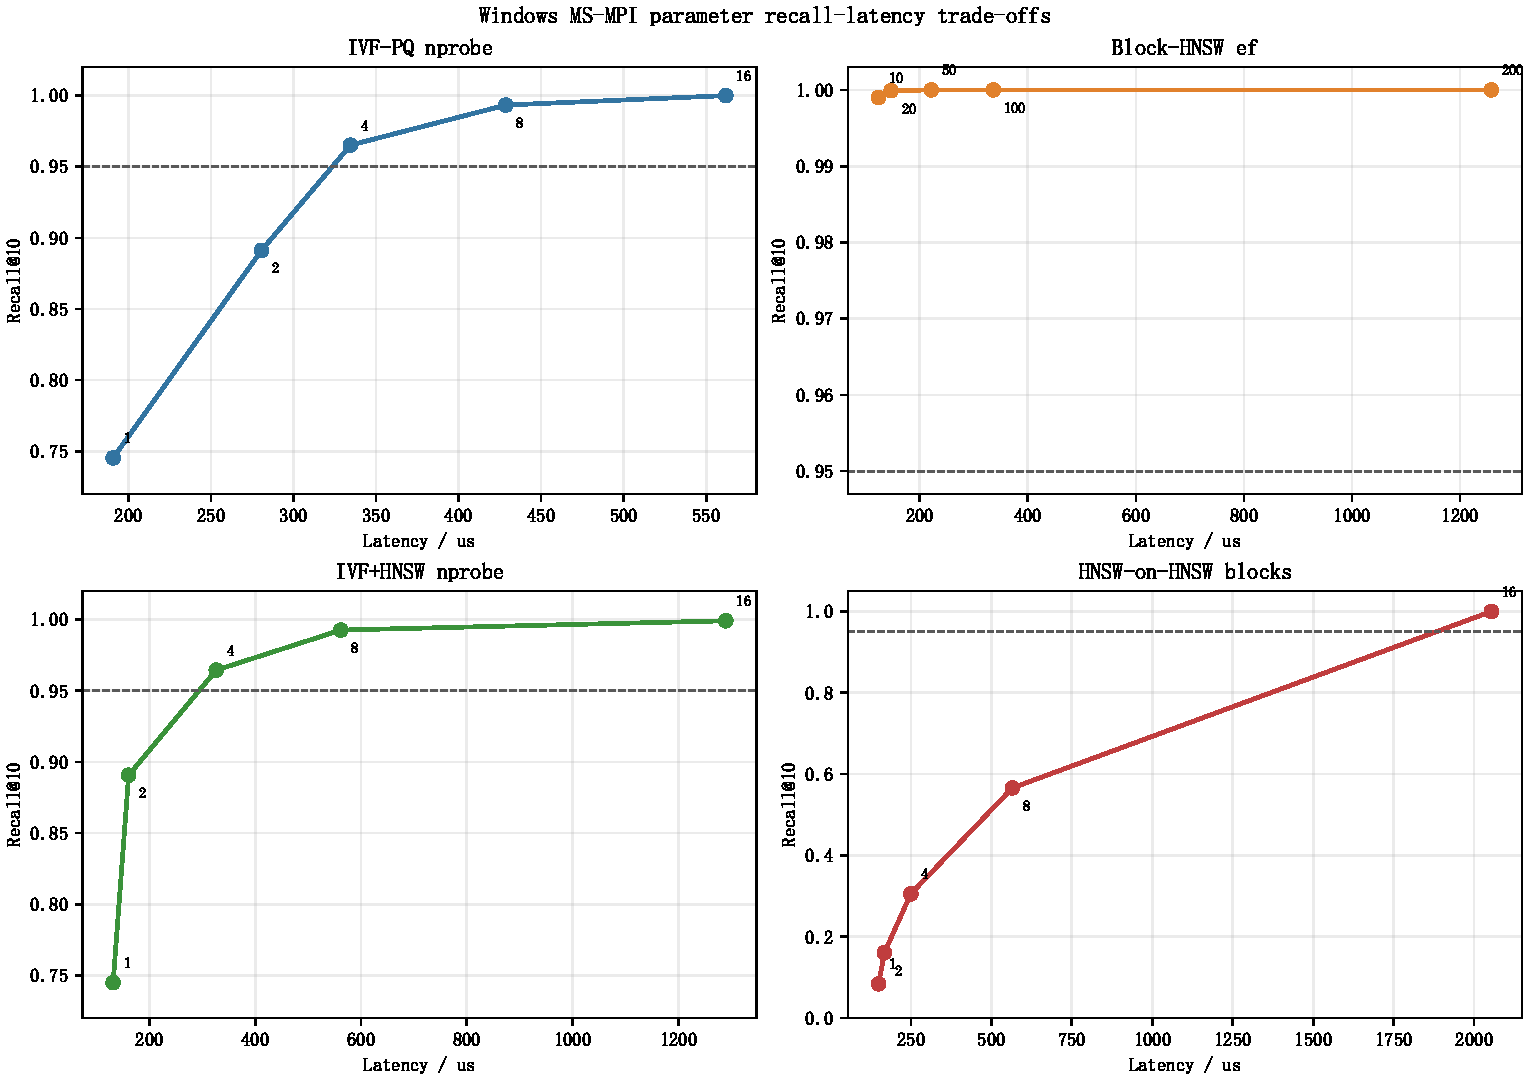
\includegraphics[width=0.96\textwidth]{mpi_parameter_tradeoffs.pdf}
  \caption{Windows MS-MPI 参数扫描的 Recall-Latency 曲线。每个子图对应一种算法的核心参数。}
  \label{fig:param_windows}
\end{figure}

\subsubsection{双平台参数曲线}

图 \ref{fig:param_cross} 将同一组参数曲线放到 Windows 与鲲鹏 PBS 两个平台比较。两平台曲线在纵轴上几乎重合，参数对召回的影响由算法结构主导；横轴位置不同，来自硬件、MPI runtime 和服务器队列环境对绝对延迟的影响。因此后续表格同时保留 recall 和 latency，避免把返回质量与性能代价混在一起。

\begin{figure}[H]
  \centering
  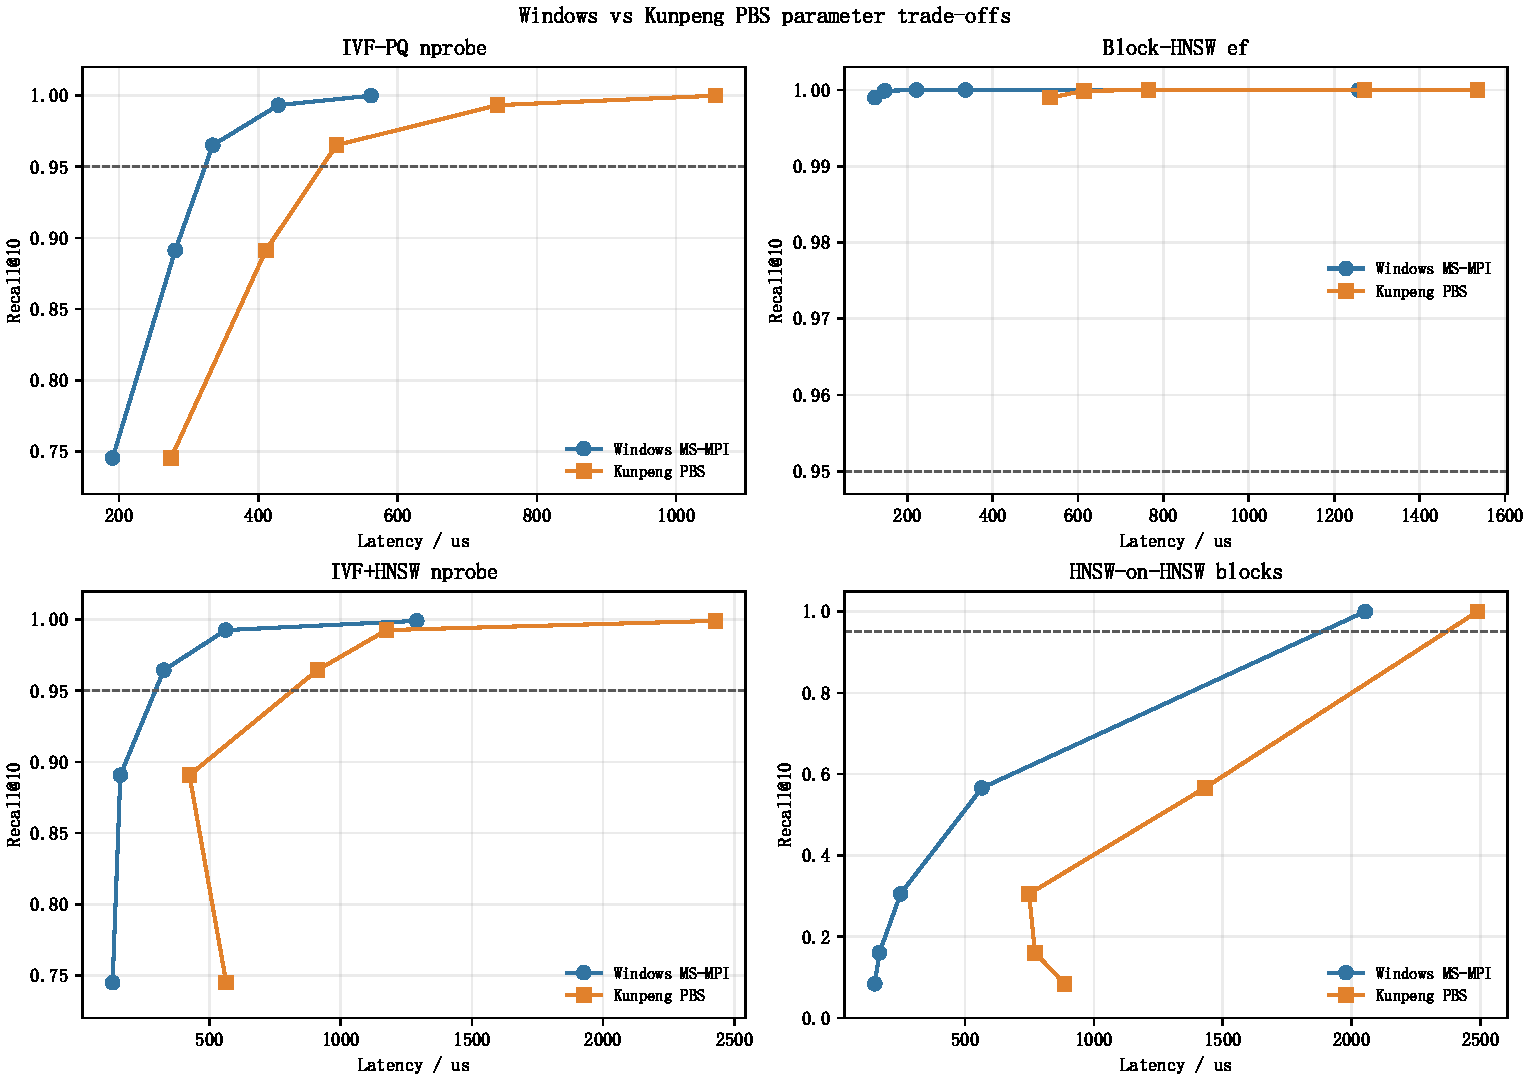
\includegraphics[width=0.96\textwidth]{mpi_cross_platform_tradeoffs.pdf}
  \caption{Windows MS-MPI 与 Kunpeng PBS 的参数 trade-off 对比。}
  \label{fig:param_cross}
\end{figure}

\subsubsection{IVF-PQ 的 nlist 影响}

IVF-PQ 额外扫描了 \code{nlist=8,16,32,64}。图 \ref{fig:nlist} 固定 \code{nprobe=4}，观察粗聚类数量变化。较小 \code{nlist} 会让每个 inverted list 更长，单次探测扫描更多向量；较大 \code{nlist} 会降低每个 list 长度，但也可能使同样 \code{nprobe} 覆盖的全局空间变窄。实验中 \code{nlist=16,nprobe=4} 是召回和延迟较均衡的代表配置。

\begin{figure}[H]
  \centering
  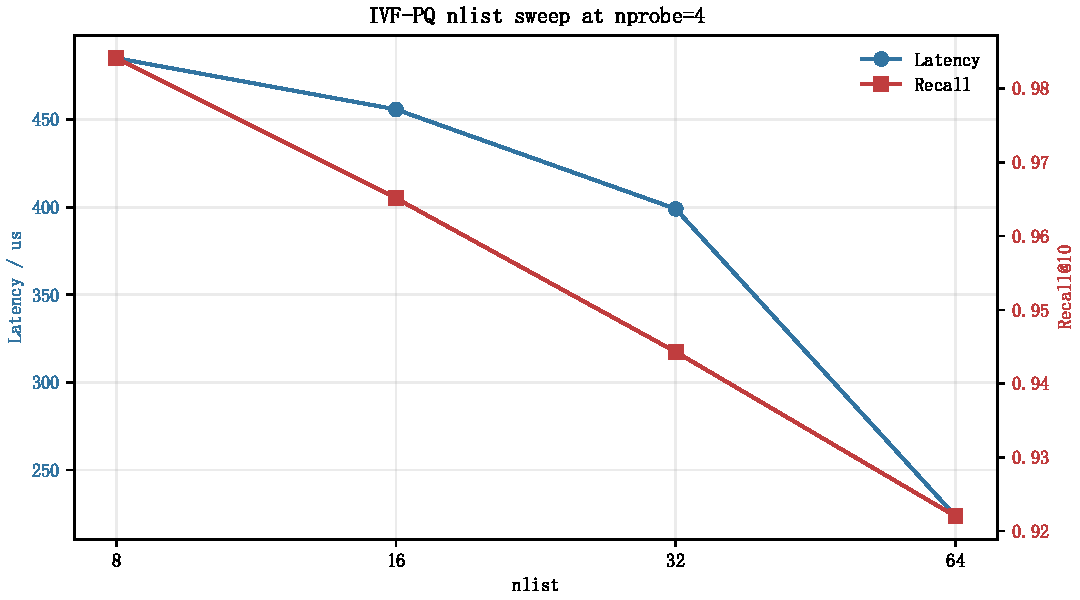
\includegraphics[width=0.72\textwidth]{mpi_ivfpq_nlist_sweep.pdf}
  \caption{IVF-PQ 在 \code{nprobe=4} 下的 \code{nlist} sweep。}
  \label{fig:nlist}
\end{figure}

\subsubsection{参数选择建议}

参数扫描给出以下取舍。IVF-PQ 若追求 Recall@10 约 0.96，\code{nlist=16}、\code{nprobe=4}、\code{p=1000} 是本次实验采用的代表配置；继续增加 \code{nprobe} 时，召回提升变小而延迟增加。Block-HNSW 在 \code{ef=50} 时已达到 Recall@10=1.00000，适合作为高召回图索引方案。IVF+HNSW 的召回受粗聚类筛选影响，\code{nprobe} 太小时即使簇内 HNSW 足够精确也无法恢复漏掉的真实近邻。HNSW-on-HNSW 验证了分层图结构；若把它作为低延迟方案，需要减少 \code{nprobe_blocks} 并接受召回下降。

\subsection{与串行基线的对比：从 SIMD、多线程到 MPI}

前两次 ANN 实验已经留下两条基线。第一条是最原始的串行 Flat 全扫描，它保持 exact top-$k$，适合衡量“从串行精确扫描到 ANN 索引加并行”的累计收益；第二条是同一索引族的单线程实现，它更适合判断本次 MPI 迁移是否继续降低了延迟。表 \ref{tab:serial_baseline_speedup} 同时列出 Windows i9 与鲲鹏 PBS；表内加速比只在同一平台内计算，不跨平台相除。

\begin{table}[H]
  \centering\footnotesize\setlength{\tabcolsep}{3.2pt}
  \begin{tabular}{p{1.75cm}p{3.35cm}C{1.25cm}C{1.55cm}C{1.35cm}C{1.35cm}}
    \toprule
    平台 & 配置 & Recall & latency & Flat 基线 & 同族 1T \\
    \midrule
    Windows & Flat 串行 & 0.99995 & 4571.62 & 1.00$\times$ & 1.00$\times$ \\
    Windows & Flat-AVX2 & 0.99995 & 1756.11 & 2.60$\times$ & 2.60$\times$ \\
    Windows & IVF-PQ 1T local & 0.95945 & 666.25 & 6.86$\times$ & 1.00$\times$ \\
    Windows & MPI IVF-PQ 4x2 & 0.96560 & 232.45 & 19.67$\times$ & 2.87$\times$ \\
    Windows & HNSW 1T baseline & 0.96865 & 65.48 & 69.82$\times$ & 1.00$\times$ \\
    Windows & MPI Block-HNSW 8x2 & 1.00000 & 195.11 & 23.43$\times$ & 0.34$\times$ \\
    \midrule
    鲲鹏 PBS & Flat 串行 & 0.99995 & 16120.74 & 1.00$\times$ & 1.00$\times$ \\
    鲲鹏 PBS & Flat-NEON & 0.99995 & 5821.16 & 2.77$\times$ & 2.77$\times$ \\
    鲲鹏 PBS & IVF-PQ 1T local & 0.95970 & 1011.89 & 15.93$\times$ & 1.00$\times$ \\
    鲲鹏 PBS & MPI IVF-PQ 4x2 & 0.96560 & 311.45 & 51.76$\times$ & 3.25$\times$ \\
    鲲鹏 PBS & HNSW 1T baseline & 0.96865 & 357.81 & 45.05$\times$ & 1.00$\times$ \\
    鲲鹏 PBS & MPI Block-HNSW 4x2 & 1.00000 & 248.00 & 65.00$\times$ & 1.44$\times$ \\
    \bottomrule
  \end{tabular}
  \caption{双平台相对原始串行 Flat 与同族单线程基线的对比。延迟单位为 $\mu$s/query；Flat 行来自 SIMD 实验，IVF-PQ/HNSW 单线程行来自 Pthread/OpenMP 实验，MPI 行来自本实验强扩展结果。}
  \label{tab:serial_baseline_speedup}
\end{table}

这张表不能被读成单一的“MPI 加速比排行榜”。相对 Flat 串行的数字包含了索引近似、SIMD 距离内核、线程并行和 MPI shard 划分的共同收益；相对同族 1T 的数字才更接近并行化本身。IVF-PQ 在两平台上都能从 MPI 切分中继续受益，Windows 为 $2.87\times$，鲲鹏为 $3.25\times$；Block-HNSW 的差异更能说明平台影响：Windows 上本地 HNSW 1T 已很快，MPI 高召回点慢于该基线，而鲲鹏上 Block-HNSW 4x2 比本地 HNSW 1T 快 $1.44\times$。原因不在 Recall，表 \ref{tab:default_points} 已显示两平台 Recall 一致；主要差异来自 SIMD 宽度、频率、MPI runtime/队列环境，以及图索引在 ARM 服务器上更明显的内存访问和负载尾部。

\subsection{强扩展：什么时候更多 rank 不再有益}

强扩展实验验证的是 owner-computes 设计的另一面：rank 变多会让每个局部索引更小，但候选 gather、同步等待和 rank 间尾部也会变重。上一节已经给出与串行 Flat 和同族 1T 的对比；本节的 speedup 与效率改以同一算法的 \code{np=1,threads=2} 为基准，只改变 MPI 进程数。这个基线是单 MPI 进程加两个 OpenMP 线程，不是纯串行单线程程序。该口径用于隔离“进程数变化”的影响，同时保持 rank 内 OpenMP 内核与正式提交配置一致。表 \ref{tab:scale_matrix} 也用同样口径列出扩展性矩阵。

\subsubsection{Windows 强扩展}

图 \ref{fig:scalability_windows} 给出 Windows 上 \code{np=1,2,4,8} 的加速比和并行效率。IVF-PQ 在 4 个进程时达到 $1.30\times$，但 8 个进程回落到 $0.99\times$；IVF+HNSW 在 2 个进程时达到 $1.32\times$，之后因为本地图搜索变短而通信、调度和索引常数项占比上升。Block-HNSW 和 HNSW-on-HNSW 在 Windows 上没有线性加速，图搜索的局部结构、内存访问和进程启动/通信成本抵消了 shard 变小带来的收益。

\begin{figure}[H]
  \centering
  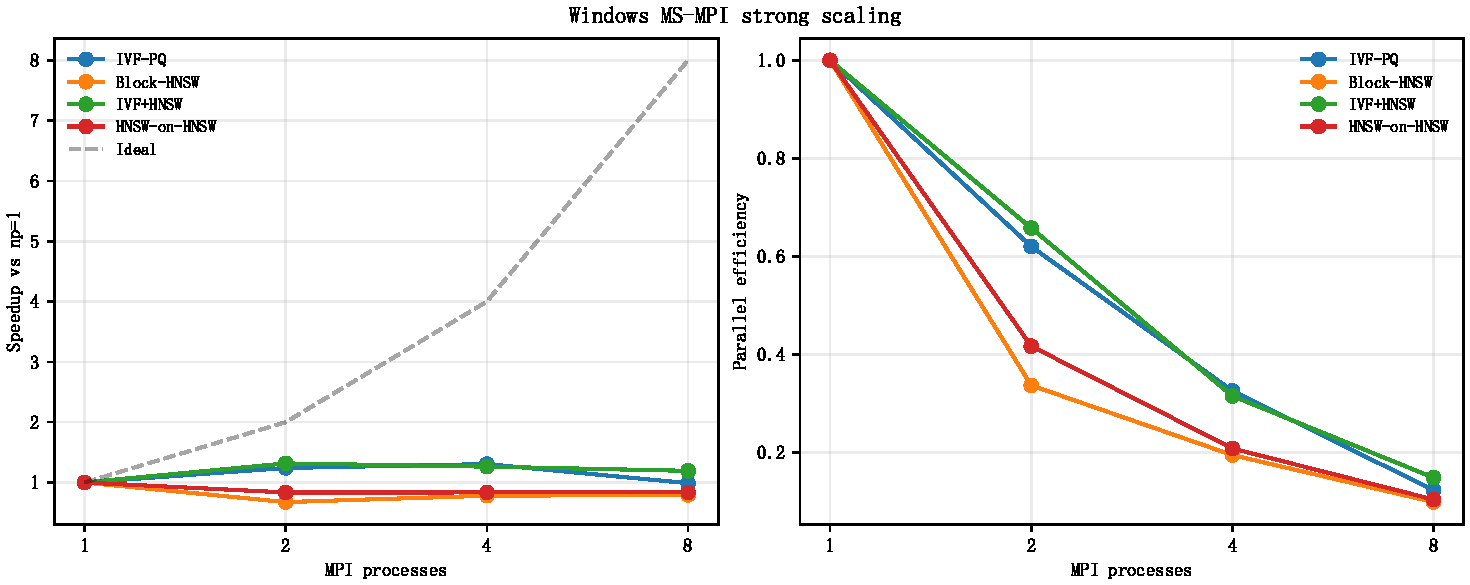
\includegraphics[width=0.95\textwidth]{mpi_scalability.pdf}
  \caption{Windows MS-MPI 强扩展：相对 \code{np=1,threads=2} 混合基线的加速比与并行效率。}
  \label{fig:scalability_windows}
\end{figure}

\subsubsection{双平台扩展性}

图 \ref{fig:scalability_cross} 直接比较两平台的延迟曲线。鲲鹏 PBS 上 IVF-PQ 从 \code{np=1} 的 571.67 $\mu$s 降到 \code{np=4} 的 311.45 $\mu$s，随后 \code{np=8} 回升到 532.36 $\mu$s；Block-HNSW 从 \code{np=1} 的 341.73 $\mu$s 降到 \code{np=4} 的 248.00 $\mu$s，但 \code{np=8} 上升到 776.99 $\mu$s。在当前数据量和 query batch 下，增加进程数并不总是等价于更快：当每个 rank 的本地任务过小，固定通信、合并、调度、HNSW 图构建差异和节点负载噪声会更突出。

\begin{figure}[H]
  \centering
  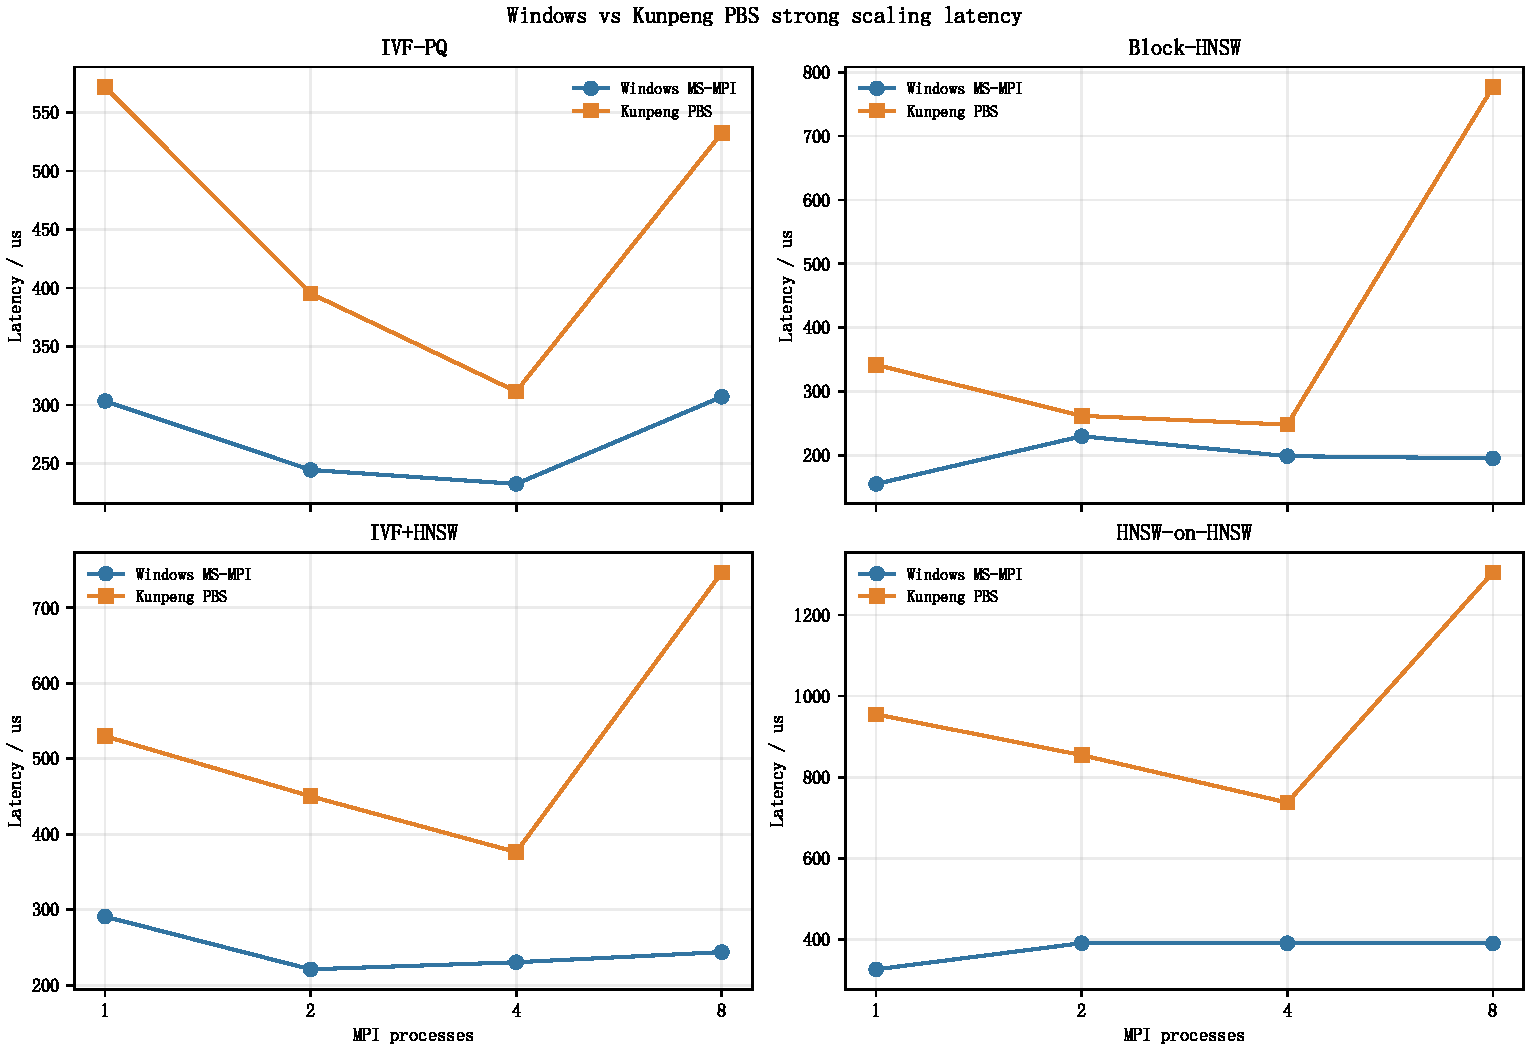
\includegraphics[width=0.96\textwidth]{mpi_cross_platform_scalability.pdf}
  \caption{Windows MS-MPI 与 Kunpeng PBS 的强扩展延迟曲线。}
  \label{fig:scalability_cross}
\end{figure}

\subsubsection{扩展性数据表}

表 \ref{tab:scaling_summary} 汇总两平台每个算法的最好进程数。从结果看，IVF-PQ 在两平台都在 4 个进程附近最好；Block-HNSW 在鲲鹏 PBS 的 4 个进程最好，但 Windows 上单进程更快；IVF+HNSW 在 Windows 上 2 个进程最好，在鲲鹏上 4 个进程最好；HNSW-on-HNSW 在 Windows 上单进程最好，在鲲鹏上 4 个进程最好。

\begin{table}[H]
  \centering\small
  \begin{tabular}{p{3.0cm}p{3.0cm}C{1.5cm}C{1.8cm}C{1.8cm}C{1.8cm}}
    \toprule
    平台 & 算法 & 最佳 np & 最低延迟 & np=8 延迟 & np=8 效率 \\
    \midrule
    Windows & IVF-PQ & 4 & 232.45 & 306.91 & 0.12 \\
    Windows & Block-HNSW & 1 & 155.03 & 195.11 & 0.10 \\
    Windows & IVF+HNSW & 2 & 221.06 & 243.89 & 0.15 \\
    Windows & HNSW-on-HNSW & 1 & 325.77 & 389.81 & 0.10 \\
    \midrule
    鲲鹏 PBS & IVF-PQ & 4 & 311.45 & 532.36 & 0.13 \\
    鲲鹏 PBS & Block-HNSW & 4 & 248.00 & 776.99 & 0.05 \\
    鲲鹏 PBS & IVF+HNSW & 4 & 376.36 & 746.84 & 0.09 \\
    鲲鹏 PBS & HNSW-on-HNSW & 4 & 737.31 & 1305.40 & 0.09 \\
    \bottomrule
  \end{tabular}
  \caption{强扩展实验摘要。延迟单位为 $\mu$s/query，效率以同算法 \code{np=1,threads=2} 为基准。表 \ref{tab:default_points} 的代表点固定为 \code{np=8,threads=2}，本表则列出同一扩展性矩阵中的最低延迟点。}
  \label{tab:scaling_summary}
\end{table}

\subsubsection{Amdahl 视角}

用 Amdahl 定律估计并行效率时，可将不可扩展部分粗略视为通信、merge、同步、调度和无法随 shard 缩小线性下降的图遍历常数项。这里的 $S_4$ 仍然相对 \code{np=1,threads=2} 混合基线，而非纯串行程序；因此下式得到的是“混合基线下的有效不可扩展比例”。设 \code{np=4} 的速度提升为 $S_4$，则
\[
\alpha \approx \frac{1/S_4-1/4}{1-1/4}.
\]
鲲鹏 PBS 上 IVF-PQ 的 $S_4=571.67/311.45=1.84$，得到 $\alpha\approx0.39$；Windows IVF-PQ 的 $S_4=303.31/232.45=1.30$，得到 $\alpha\approx0.69$。这个估计不能解释为算法的纯串行比例，因为 \code{np=1} 已含两个 OpenMP 线程；它把小规模 shard 下的额外成本、OpenMP 基线和 MPI 固定开销都折算进“不可扩展部分”。在 100K base、2000 query 的规模下，MPI 强扩展已经不是理想均匀计算模型，通信和运行时常数需要与本地搜索一起考虑。

\subsubsection{MPI/OpenMP 混合布局}

前面的强扩展实验固定 \code{threads=2}，只改变 MPI 进程数。为了更接近实际调参过程，本节在 Windows MS-MPI 上进一步固定总 worker 预算，比较 \code{np} $\times$ \code{threads} 的不同分配方式。实验覆盖 8 个 worker 下的 \code{1x8}、\code{2x4}、\code{4x2}、\code{8x1}，以及 16 个 worker 下的 \code{1x16}、\code{2x8}、\code{4x4}、\code{8x2}。HNSW-on-HNSW 在本节固定 \code{nprobe_blocks=4}，用于观察布局对调度和访存的影响；高召回配置仍以前文 \code{nprobe_blocks=16} 的参数扫描结果为准。

\begin{figure}[H]
  \centering
  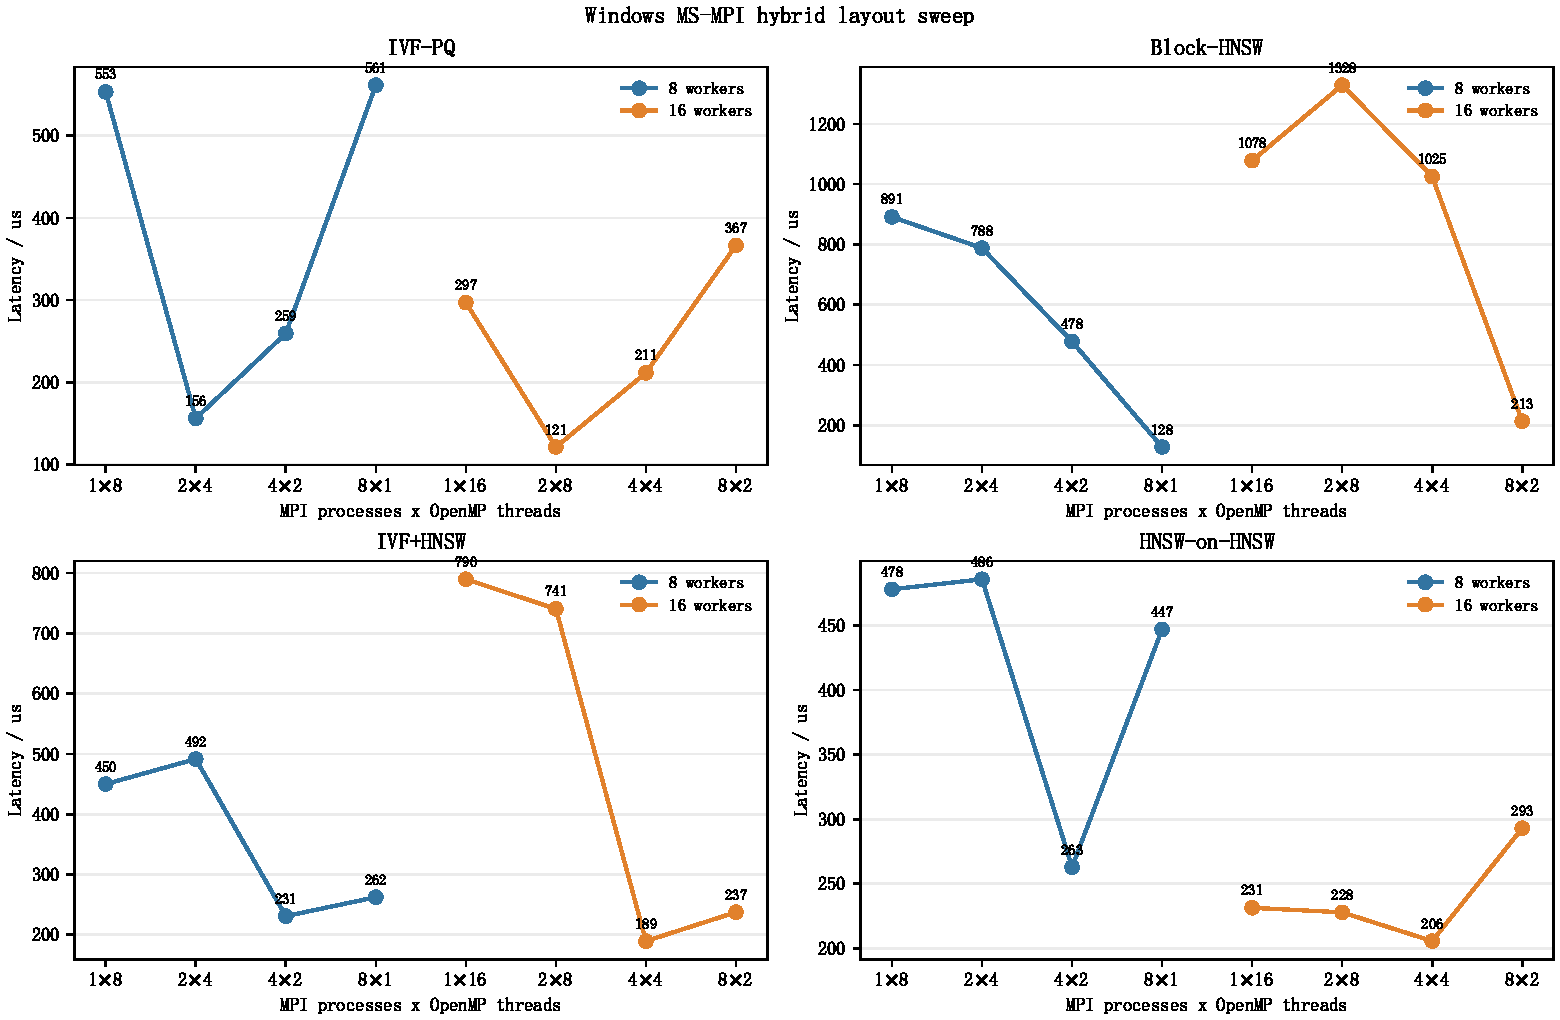
\includegraphics[width=0.96\textwidth]{mpi_hybrid_layout.pdf}
  \caption{Windows MS-MPI 上固定 worker 预算的 \code{np} $\times$ \code{threads} 布局实验。}
  \label{fig:hybrid_layout}
\end{figure}

图 \ref{fig:hybrid_layout} 显示，不同算法适合的布局并不相同。IVF-PQ 在 16 worker 预算下以 \code{2x8} 最快，延迟为 121.23 $\mu$s/query；它既保留了 MPI shard 缩小带来的扫描减少，也让每个 rank 内仍有足够线程处理倒排表。Block-HNSW 更偏向更多 MPI shard，8 worker 下 \code{8x1} 达到 128.05 $\mu$s/query，图搜索中的 rank 内并行收益有限，缩小本地图规模更直接。IVF+HNSW 的最好点是 \code{4x4}，延迟为 189.48 $\mu$s/query，介于倒排筛选和图遍历之间。HNSW-on-HNSW 在该中等探测配置下也是 \code{4x4} 最稳，过多 rank 会增加 top-level block 选择和候选合并的尾部。

\subsubsection{Windows 亲和性实验}

本地 Windows 平台是 P-core/E-core 混合架构。为了检查运行时调度对 MPI 作业的影响，本节使用同一个 MPI 二进制、同一组 \code{np=4,threads=2,query_n=2000} 参数，通过 \code{cmd /AFFINITY} 分别测试默认调度、仅 P-core、仅 E-core，以及 P/E 全开。该实验仍然是真实 MS-MPI 运行，只改变进程可见的逻辑核集合。

\begin{figure}[H]
  \centering
  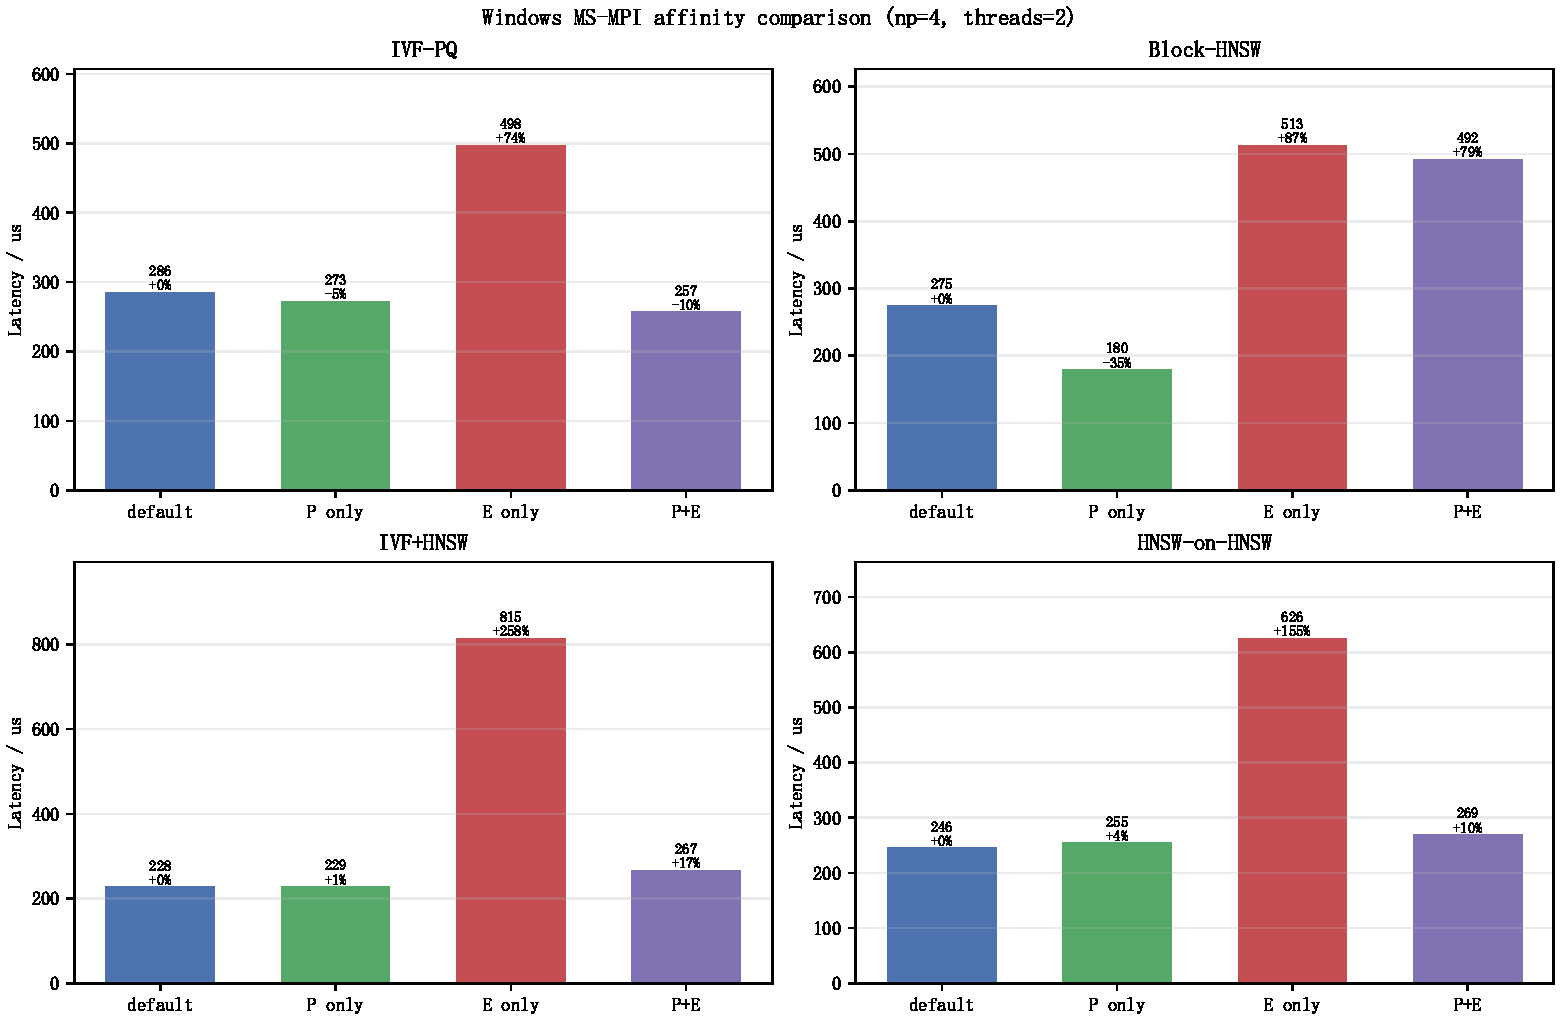
\includegraphics[width=0.96\textwidth]{mpi_affinity.pdf}
  \caption{Windows MS-MPI 亲和性实验，固定 \code{np=4,threads=2}。}
  \label{fig:affinity}
\end{figure}

E-core-only 对所有算法都变慢，IVF+HNSW 从默认的 227.71 $\mu$s/query 增加到 814.81 $\mu$s/query，HNSW-on-HNSW 也增加到 625.63 $\mu$s/query；后文 VTune uarch 中，E-core Back-End Bound 与 Memory Bound 分别达到 60.1\% 和 50.4\%。P-core-only 对 Block-HNSW 最有帮助，延迟从 274.61 降到 179.60 $\mu$s/query；IVF-PQ 则在 P/E 全开时最快，规则扫描和多 rank 并发能利用更多逻辑核。正式跨平台结果保留默认调度，亲和性实验用于解释本地波动和混合架构影响。

\subsection{通信与负载：验证 MPI 边界是否选对}

如果算法设计章节中的固定长度候选协议是合适的，那么通信/merge 应该只表现为小的固定项，真正拉开延迟的是每个 rank 的本地搜索时间和最慢 rank 的尾部。本节用通信占比、per-rank 搜索时间和 base shuffle 对照来检查这一点。

\subsubsection{通信与 merge 随进程数变化}

图 \ref{fig:comm_balance} 左侧展示通信与 merge 开销随进程数的变化。两平台日志都显示 \code{comm+merge latency} 从 \code{np=1} 到 \code{np=8} 增大，但绝对值只有微秒级。以鲲鹏 PBS 为例，\code{np=8} 下 IVF-PQ 的通信/merge 为 2.88 $\mu$s，Block-HNSW 为 2.55 $\mu$s，IVF+HNSW 为 3.37 $\mu$s，HNSW-on-HNSW 为 3.05 $\mu$s。与数百到上千微秒的本地搜索相比，这部分还不是主瓶颈。

\begin{figure}[H]
  \centering
  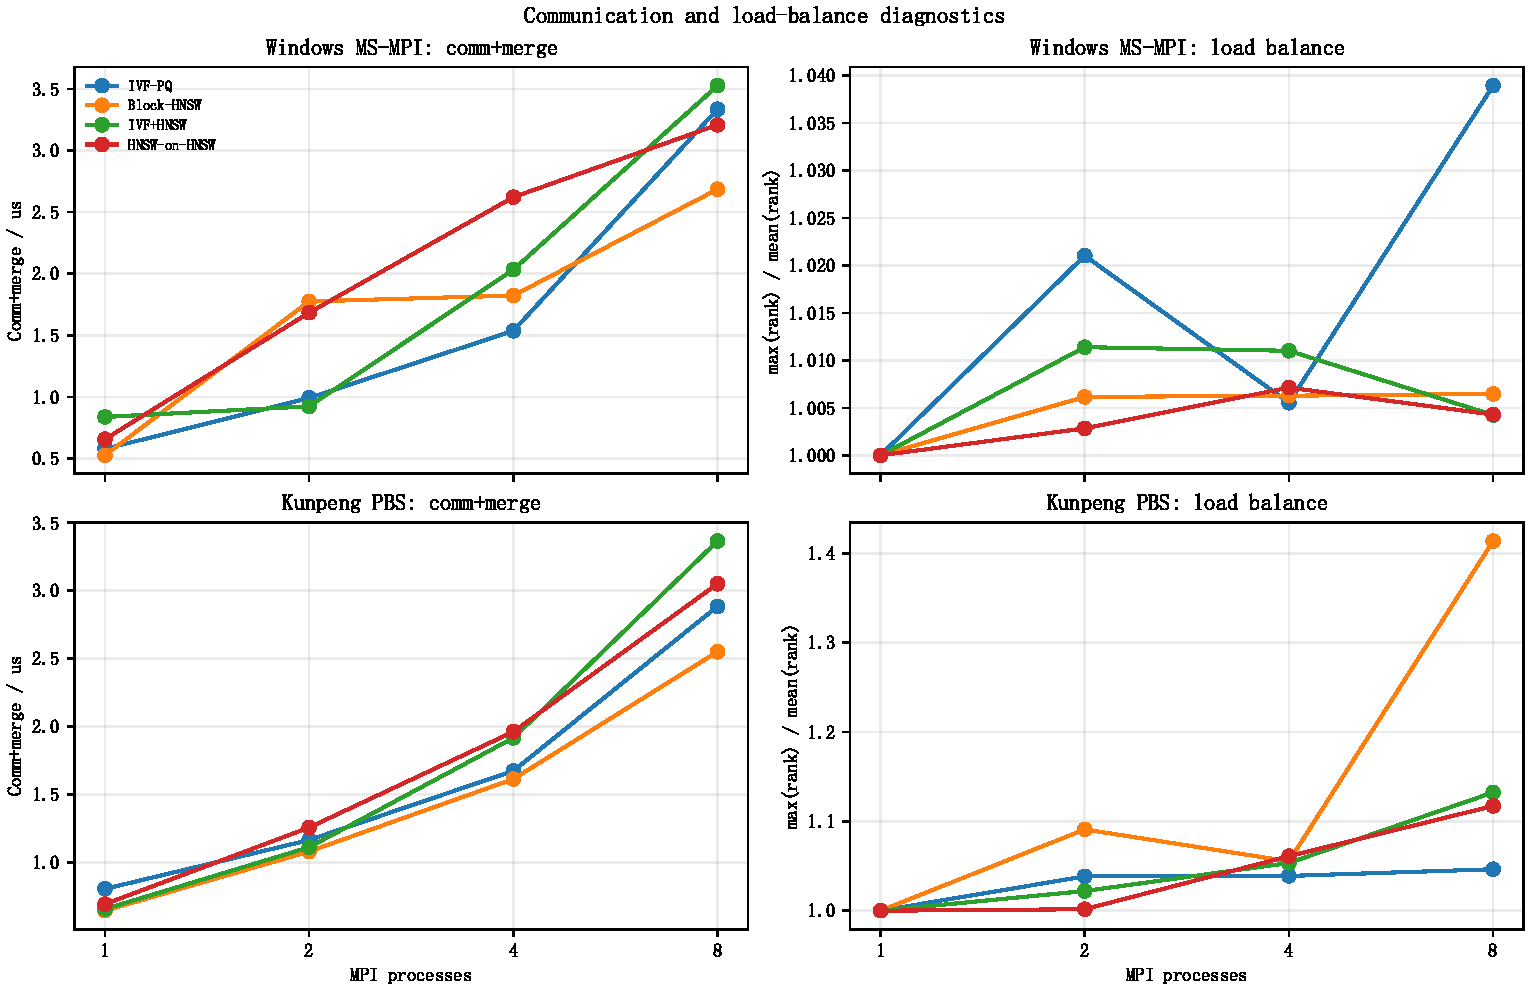
\includegraphics[width=0.95\textwidth]{mpi_comm_balance.pdf}
  \caption{通信/merge 开销与 rank 负载不均衡度。}
  \label{fig:comm_balance}
\end{figure}

\subsubsection{通信占比}

表 \ref{tab:comm_ratio} 使用代表参数点计算通信与 merge 占总延迟比例。Windows 上四种算法在 0.37\%--1.20\% 之间，鲲鹏 PBS 上四种算法均不超过 0.53\%。在当前规模中，优化方向应优先放在本地索引结构和 rank 内搜索，通信拓扑重写的收益空间较小。

\begin{table}[H]
  \centering\small
  \begin{tabular}{p{3.1cm}C{2.1cm}C{2.1cm}C{2.1cm}C{2.1cm}}
    \toprule
    平台 & IVF-PQ & Block-HNSW & IVF+HNSW & HNSW-on-HNSW \\
    \midrule
    Windows MS-MPI & 1.04\% & 1.20\% & 1.11\% & 0.37\% \\
    鲲鹏 PBS & 0.53\% & 0.34\% & 0.33\% & 0.12\% \\
    \bottomrule
  \end{tabular}
  \caption{代表参数点中通信与 merge 占平均总延迟比例}
  \label{tab:comm_ratio}
\end{table}

\subsubsection{负载不均衡分析}

负载不均衡度采用 $\max(T_i)/\mathrm{mean}(T_i)$。Windows 上代表参数点均低于 1.07，本地机器的各 rank 搜索时间比较接近。鲲鹏 PBS 上图索引的不均衡更明显：代表参数点中 Block-HNSW 为 1.19441，HNSW-on-HNSW 为 1.17062；扩展性实验 \code{np=8} 时 Block-HNSW 甚至达到 1.41。图搜索路径与数据分布有关，即使 base 数量均分，不同 rank 的图遍历代价仍可能不同。

从算法结构看，IVF-PQ 的扫描量由 selected list 长度决定，list 长度不均会引入尾部；Block-HNSW 的搜索路径由图邻接和 query 位置决定，某些 shard 可能需要扩展更多节点；IVF+HNSW 同时受聚类和图搜索影响；HNSW-on-HNSW 又加入了 top-level block 选择，若探测全部 block，负载更接近 block 内图搜索总和。

\subsubsection{随机打散 base 的实证}

为验证负载均衡判断，程序增加了构建前随机打散 base 的路径。设置
\begin{lstlisting}[language=bash]
USE_SHUFFLED_BASE=1
BASE_SHUFFLE_SEED=20260525
\end{lstlisting}
后，rank 0 先用固定 seed 打乱 base 向量和原始全局 id，再分别 \code{MPI_Scatterv} 给各 rank。本地搜索仍只看连续内存 shard；候选打包时通过同步散发的 \code{local_global_ids} 把本地 id 映射回原始 id，因此 Recall 仍可直接和 ground truth 对齐。未设置该开关时仍保留连续切分，作为正文主结果和对照组。

\begin{table}[H]
  \centering\footnotesize
  \begin{tabular}{p{2.8cm}C{1.7cm}C{1.9cm}C{1.9cm}C{1.9cm}C{1.5cm}}
    \toprule
    平台 & base & latency & local max & imbalance & Recall \\
    \midrule
    Windows MS-MPI & 连续 & 219.80120 & 216.95125 & 1.00781 & 1.00000 \\
    Windows MS-MPI & 打散 & 222.93255 & 220.35495 & 1.00581 & 1.00000 \\
    鲲鹏 PBS & 连续 & 781.51286 & 778.25868 & 1.06455 & 1.00000 \\
    鲲鹏 PBS & 打散 & 769.51754 & 766.40415 & 1.01648 & 1.00000 \\
    \bottomrule
  \end{tabular}
  \caption{Block-HNSW 在 \code{np=8,threads=2,ef=50,query_n=2000} 下的 base 打散对比。延迟单位为 $\mu$s/query。}
  \label{tab:base_shuffle}
\end{table}

表 \ref{tab:base_shuffle} 中 Windows 原本已经接近平衡，打散只把 imbalance 从 1.00781 降到 1.00581，延迟差异主要落在运行噪声内。鲲鹏 PBS 的同一作业中效果更明显：rank 最慢/平均比从 1.06455 降到 1.01648，平均延迟从 781.51286 降到 769.51754 $\mu$s/query。结合前述旧扩展性日志中 \code{np=8} 曾出现的 1.41364，随机打散不能消除所有调度和图遍历波动，但能降低“某个连续 shard 明显更难搜”的尾部风险。list 粒度重分配、按历史时间拆分慢 rank 仍属于更细的后续均衡策略。

\subsection{本地搜索瓶颈：从图遍历原理到 VTune 证据}

前几节已经看到通信不是主要开销；如果报告只停在“本地搜索慢”，设计结论仍然不够可解释。因此这里把 rank 内 HNSW 搜索抽象成三层瓶颈：距离内核、图遍历、候选队列。VTune 采集使用与 MPI rank 内相同的搜索内核，但关闭 MPI 包装，只用于解释本地搜索内部结构；真实端到端延迟仍以前文 MPI 实验为准，完整命令、汇编摘录和硬件事件表移到附录 \ref{sec:appendix_vtune}。

\begin{table}[H]
  \centering\small
  \begin{tabularx}{\textwidth}{p{3.0cm}p{4.7cm}Y}
    \toprule
    观察层次 & 关键结果 & 对优化的影响 \\
    \midrule
    Hotspots & CPU Time 为 19.922 s，其中 \code{_mm256_mul_ps} wrapper 占 16.2\%，\code{searchBaseLayer} 占 12.5\%，\code{pthread_mutex_lock} 占 13.4\%。 & 距离计算仍频繁出现，但它和图遍历、候选队列、runtime 同步交织在一起。\\
    指令层 & AVX 内积循环每轮处理 16 个 \code{float}，DEEP100K 的 96 维向量正好对应 6 个 AVX 块。 & 距离内核已经向量化，主要问题在于 SIMD kernel 被不规则访问包围。\\
    微架构层 & E-core Back-End Bound 为 60.1\%，Memory Bound 为 50.4\%，DRAM Bound 为 30.1\%。 & 后端和内存层次是主要限制，visited 标记、邻接表和向量地址访问会带来 TLB/DRAM 压力。\\
    \bottomrule
  \end{tabularx}
  \caption{本地 HNSW 搜索瓶颈摘要，细节见附录 \ref{sec:appendix_vtune}}
  \label{tab:vtune_body}
\end{table}

这些数据把“本地搜索主导延迟”进一步落到 HNSW 的运行机制上：高召回来自沿图邻居逐步扩展，rank 需要不断维护候选队列、检查 visited 标记、比较优先级并访问分散的向量地址。距离函数本身已经走 AVX 路径，但它不是一个连续大数组扫描 kernel，而是嵌在 query 相关的图遍历中。因此后续优化应优先改善 rank 内图访问局部性、减少候选队列维护成本，并降低慢 shard 带来的尾部等待。

\subsection{通信范式：非阻塞收益取决于数据流}

在当前架构中，通信模式是 MPI 外壳的一部分，可以在不改变本地索引的情况下切换。默认路径使用阻塞 \code{MPI_Bcast} 与 gather；补充路径把 gather 改为 \code{MPI_Igather} 并在候选真正需要前 \code{MPI_Wait}。本节考察当前数据流里是否存在足够的计算/通信重叠空间；非阻塞 API 本身不会增加新的本地搜索并行度。

表 \ref{tab:comm_modes} 给出鲲鹏 PBS 的结果。四种算法的 Recall 在阻塞与非阻塞模式下完全一致；性能上，IVF-PQ 和 IVF+HNSW 有 5\% 到 6\% 的改善，Block-HNSW 基本持平，HNSW-on-HNSW 则略慢。非阻塞通信在本实现中可以正常使用，但收益不稳定，受各 rank 本地搜索结束时间差、runtime 调度和 gather 数据到达节奏影响。

\begin{table}[H]
  \centering\small
  \begin{tabular}{p{3.2cm}C{2.1cm}C{2.3cm}C{2.0cm}C{2.1cm}}
    \toprule
    算法 & Blocking & Nonblocking & 变化 & Recall \\
    \midrule
    IVF-PQ & 594.79821 & 564.27193 & -5.13\% & 0.96515 \\
    Block-HNSW & 812.47854 & 808.22515 & -0.52\% & 1.00000 \\
    IVF+HNSW & 961.82323 & 900.58351 & -6.37\% & 0.96450 \\
    HNSW-on-HNSW & 2335.40905 & 2356.10485 & +0.89\% & 0.99995 \\
    \bottomrule
  \end{tabular}
  \caption{鲲鹏 PBS 阻塞/非阻塞通信模式对比。延迟单位为 $\mu$s/query。}
  \label{tab:comm_modes}
\end{table}

MPI 线程级别方面，本程序使用 \code{MPI_Init_thread}，默认请求 \code{MPI_THREAD_FUNNELED}；OpenMP worker 只做 rank 内搜索，只有主线程调用 MPI，因此该级别已经满足正确性。补充实验显示 Windows MS-MPI 与鲲鹏 PBS 都能提供 \code{MPI_THREAD_MULTIPLE}，Recall 不变，但延迟变化一正一负，详细表格见附录 \ref{sec:appendix_comm_detail}。因此 \code{MULTIPLE} 在本程序中主要是编程范式覆盖，不是必要优化。

单边通信（RMA）也可以映射到当前候选协议：rank 0 建立 \code{MPI_Win}，其他 rank 用 \code{MPI_Put} 或 rank 0 用 \code{MPI_Get} 取回固定长度候选块。问题在于 RMA 仍需要窗口同步，也无法减少 $QPk$ 个候选的总传输量。由于表 \ref{tab:comm_ratio} 中通信/merge 占比最高只有 1.20\%，当前阶段更值得投入的是 tile 化流水线：当 tile $i$ 的候选在后台 gather 时，rank 搜索 tile $i+1$。这会改变 query batch 和 merge 缓冲结构，因此 RMA 只作为后续方向，不在当前结果中宣称加速。

\section{综合讨论}

\subsection{设计复盘：哪些决策被证据支持}

\textbf{局部候选协议是可靠边界。}四种模式在 Windows MS-MPI 与鲲鹏 PBS 中的代表参数 Recall 完全一致，尤其是 IVF-PQ 的 0.96515、IVF+HNSW 的 0.96450、Block-HNSW 的 1.00000 以及 HNSW-on-HNSW 的 0.99995 在两平台中一致。由此确认跨 rank 全局 id 映射、候选布局和 rank 0 merge 没有破坏 ANN 结果。

\textbf{通信不是当前首要矛盾。}代表参数中通信/merge 占比最高为 1.20\%，鲲鹏 PBS 上最高为 0.53\%。这验证了固定长度 top-$k$ 候选协议的价值：MPI 层的成本被控制住后，优化重点应转向 rank 内索引结构、图访问局部性和负载尾部。

\textbf{更多 rank 不等于更快。}强扩展结果显示 \code{np=4} 通常比 \code{np=8} 更稳。这并不否定 MPI 划分，而是说明在 DEEP100K 和 2000 query 这个规模下，shard 变小带来的收益会被固定开销、进程调度和最慢 rank 等待抵消。

\textbf{高召回图索引需要关心内存行为。}Block-HNSW 在代表参数下达到满召回，但 VTune 与 uarch 事件显示图遍历、visited/TLB、DRAM 和候选队列维护才是后续优化重点。距离内核已经使用 AVX，单纯继续强调 SIMD 并不能解决 HNSW 的不规则访问问题。

详细的正确性一致性、计时一致性和脚本复现路径见附录 \ref{sec:appendix_trust} 与附录 \ref{sec:appendix_repro}。

\subsection{局限与进一步设计}

\textbf{更多重复次数。}本次已经完成全量参数扫描和扩展性实验，但每个点主要记录一次全量运行。若作为论文级 benchmark，应在服务器低负载时重复 5 次以上取中位数和四分位区间。本课程实验更关注算法和 MPI 数据流，当前日志已足以证明正确性和主要趋势。

\textbf{HNSW-on-HNSW 参数。}\code{nprobe_blocks=16} 是偏向高召回的配置，相当于在 top-level graph 之后仍搜索全部 block。本次已经扫描 \code{1,2,4,8,16} 并画出 Recall@10 与延迟曲线；若把它作为低延迟方案，还需要在 \code{4} 到 \code{16} 之间补更细粒度的探测点，寻找召回刚接近目标值时的拐点。

\textbf{更细的负载均衡。}本次已实现固定 seed 的 base 随机打散，并在鲲鹏 PBS 上把 Block-HNSW 的 imbalance 从 1.06455 压到 1.01648。它仍是静态均衡，尚未根据 inverted list 长度、HNSW 图度数或查询热度做动态重分配；如果某些 rank 长期更慢，可以继续尝试质心均衡、list 粒度分配或按历史搜索时间拆分慢 shard。

\textbf{通信优化。}当前所有候选都 gather 到 rank 0。对于更多 rank，可以改为分层合并：先在节点内合并，再跨节点合并；或者使用自定义 top-$k$ 归约。RMA 与 tile 流水线在接口上可行，但前者不减少候选总量，后者需要重写 query 批处理和 merge 缓冲；在表 \ref{tab:comm_ratio} 的通信占比下，它们不是当前首要瓶颈。

\textbf{Profiling 深度。}本次 VTune Hotspots 已用带符号二进制映射到 HNSW 搜索、AVX 内积和优先队列路径，汇编也验证了 16-float AVX 距离内核；管理员权限下的 uarch 采集进一步给出了 Back-End Bound、Memory Bound、Bad Speculation、L1/TLB 与 DRAM 指标。若继续深化，可以再做 Memory Access 分析，把具体内存对象和源码行绑定起来。

\section{结论与后续工作}

本次工作完成了 ANN 搜索从单机多线程到 MPI 多进程环境的迁移，并保留 OpenMP 作为 rank 内并行层。IVF-PQ 验证了基础倒排索引迁移；Block-HNSW、IVF+HNSW 和 HNSW-on-HNSW 分别代表三种图索引组织方式。双平台参数扫描显示，相同参数下 Recall 在 Windows 与鲲鹏 PBS 上完全一致，分布式 top-$k$ 合并逻辑正确；通信与 merge 开销在当前验证规模中很小，主要瓶颈仍是本地 ANN 搜索。

从算法效果看，IVF-PQ 与 IVF+HNSW 的召回略低但保持较好的筛选效率；Block-HNSW 在代表参数下达到 Recall@10=1.00000，是当前最可靠的高召回图索引方案；HNSW-on-HNSW 证明了分层图结构的可行性和高召回能力，但全 block 探测配置带来了明显延迟代价。强扩展实验表明，\code{np=4} 通常比 \code{np=8} 更稳，在 DEEP100K 和 2000 query 的规模下，MPI 强扩展存在固定开销与负载不均衡拐点。VTune、硬件事件与汇编分析进一步指出更具体的优化靶点：距离内核已经使用 AVX SIMD，而 E-core Back-End Bound 和 Memory Bound 分别达到 60.1\% 与 50.4\%，后续优化应集中在图遍历、候选队列、TLB/DRAM 压力和负载尾部。
\label{LastBodyPage}

\clearpage
\appendix
\setcounter{page}{1}
\renewcommand{\thepage}{A-\arabic{page}}
\cfoot{\thepage}
\section{复现与开发工具使用说明}

\subsection{工程结构与复现边界}
\label{sec:appendix_engineering}

本目录由上一阶段 ANN 多线程实验扩展而来，继续复用 SIMD、IVF、HNSW 内核。表 \ref{tab:files} 列出报告对应的主要文件。正文把这些内容放到附录，是为了让主线集中在设计原则和实验解释上；真正复现实验时，这些路径仍是源代码、日志和图表的索引。

\begin{table}[H]
  \centering\footnotesize
  \begin{tabularx}{\textwidth}{p{3.5cm}Y}
    \toprule
    文件或目录 & 作用 \\
    \midrule
    \code{main.cc} & 课程提交入口，保留 load data、distribute、build local index、search、gather、rank 0 merge 和输出指标的主流程。\\
    \code{mpi_ann_runner.h} & 聚合头文件，使服务器仍按 \code{mpic++ main.cc ...} 编译，同时把实现按模块拆分。\\
    \code{mpi/} & 保存 MPI 公共类型、参数解析、数据加载与划分、通信包装、本地搜索、候选打包/合并和输出格式模块。\\
    \code{ivf/} & 复用 IVF-PQ 索引和 OpenMP 搜索实现，作为本次 IVF 基础迁移方案。\\
    \code{hnsw/} & 保存 Block-HNSW、IVF+HNSW 和 HNSW-on-HNSW 相关实现。\\
    \code{qsub_mpi.sh} & 按提交指南启动最终代表性 PBS 作业，默认运行最快且高召回的 Block-HNSW 提交路径。\\
    \code{scripts/} & 保存 Windows 本地实验、鲲鹏 PBS 全量/补充实验自动提交、最终代表性提交、结果解析和绘图脚本。\\
    \code{results/} & 保存原始日志、解析 CSV 与 VTune 导出，所有图表数字都可回溯到这些文件。\\
    \code{report/} & 保存本报告源码、校徽资源、生成图和最终 PDF。\\
    \bottomrule
  \end{tabularx}
  \caption{ANN MPI 实验目录中的关键文件}
  \label{tab:files}
\end{table}

数据路径仍沿用前两次实验的约定：程序优先读取 \code{ANN_DATA_PATH}，服务器上设置为 \code{/anndata}，本地 Windows 脚本设置为仓库外层的 \code{files/} 数据目录。如果环境变量未设置，程序会按平台尝试默认路径。这样做避免把 DEEP100K 数据复制进提交目录，也使 Windows 与鲲鹏 PBS 两边的命令只在数据路径和作业调度上不同。

\subsection{复现命令与结果文件}
\label{sec:appendix_repro}

\subsubsection{本地复现}

\begin{lstlisting}[language=bash]
cd D:\Study\26sp\parallel\ann-mpi
make local
powershell -ExecutionPolicy Bypass -File scripts/run_parameter_sweep.ps1
powershell -ExecutionPolicy Bypass -File scripts/run_scalability.ps1
powershell -ExecutionPolicy Bypass -File scripts/run_hybrid_layout.ps1
powershell -ExecutionPolicy Bypass -File scripts/run_affinity.ps1
powershell -ExecutionPolicy Bypass -File scripts/run_final_gap_experiments.ps1
micromamba run -n test python scripts/parse_mpi_results.py
\end{lstlisting}

Windows VTune profiling 的普通 Hotspots 和管理员 uarch 采集入口如下：
\begin{lstlisting}[language=bash]
g++ main.cc -o build/main_no_mpi_profile.exe -O2 -g -std=c++11 -I. \
  -fopenmp -lpthread -mavx2 -mfma -DANN_NO_MPI
powershell -ExecutionPolicy Bypass -File scripts/run_vtune_uarch_admin.ps1
\end{lstlisting}
也可以右键管理员脚本运行；本次已导出 uarch summary、top-down、hardware events 与 hotspots 四类文件。

\subsubsection{鲲鹏 PBS 复现}

\begin{lstlisting}[language=bash]
cd ann-mpi
make clean
make
qsub qsub_mpi.sh
\end{lstlisting}
该默认提交路径对应最终上传到服务器的代表性作业：
\begin{lstlisting}[language=bash]
remote_dir=/home/s2413575/ann
job=42354.master_ubss1
NP=4
OMP_NUM_THREADS=2
\end{lstlisting}
默认 Block-HNSW 在 \code{m=16,ef=50,query_n=2000} 下得到 Recall@10=1.00000、平均延迟 236.92131 $\mu$s/query。

若需要复现实验矩阵，应提交矩阵脚本：
\begin{lstlisting}[language=bash]
qsub -v NP=8,OMP_NUM_THREADS=2,QUERY_N=2000 scripts/qsub_mpi_sweep.sh
qsub -v NP=8,OMP_NUM_THREADS=2,QUERY_N=2000 scripts/qsub_mpi_comm_modes.sh
qsub -v NP=8,OMP_NUM_THREADS=2,QUERY_N=2000 scripts/qsub_mpi_final_gaps.sh
\end{lstlisting}
最终提交脚本 \code{qsub_mpi.sh} 保持为代表性作业入口。

完整批量实验可使用自动脚本提交和回收结果：
\begin{lstlisting}[language=bash]
set KUNPENG_PASSWORD=<server_password>
micromamba run -n test python scripts/run_kunpeng_pbs_sweep_auto.py
micromamba run -n test python scripts/run_kunpeng_pbs_comm_auto.py
micromamba run -n test python scripts/run_kunpeng_pbs_final_gaps_auto.py
\end{lstlisting}

\subsubsection{生成产物}

\begin{table}[H]
  \centering\footnotesize
  \begin{tabularx}{\textwidth}{p{4.1cm}Y}
    \toprule
    文件 & 说明 \\
    \midrule
    \fcell{parameter_sweep}{20260525_141037.csv} & Windows 参数扫描结构化结果，24 行。\\
    \fcell{scalability}{20260525_145526.csv} & Windows 强扩展结构化结果，16 行。\\
    \fcell{hybrid_layout}{20260525_205224.csv} & Windows \code{np} $\times$ \code{threads} 混合布局结果，32 行。\\
    \fcell{affinity}{20260525_205832.csv} & Windows P-core/E-core 亲和性结果，16 行。\\
    \fcell{kunpeng_pbs_sweep}{20260525_153105.csv} & 鲲鹏 PBS 参数扫描与扩展性结构化结果，40 行。\\
    \fcell{kunpeng_pbs_comm_modes}{20260525_154940.csv} & 鲲鹏 PBS 阻塞/非阻塞通信模式结果，8 行。\\
    \fcell{final_gap_experiments}{20260605_210724.csv} & Windows base shuffle 与 MPI 线程级别补充结果，4 行。\\
    \fcell{kunpeng_pbs_final_gaps}{20260605_211922.csv} & 鲲鹏 PBS base shuffle 与 MPI 线程级别补充结果，4 行。\\
    \begin{tabular}[t]{@{}l@{}}\code{kunpeng_pbs}\\\code{representative}\\\code{submission}\\\code{20260606_183614.txt}\end{tabular} & 最终服务器提交验证记录，包含作业号、默认代表性算法和 \code{test.o/test.e} 摘要。\\
    \code{results/vtune_exports/*} & VTune Hotspots、汇编摘录、uarch 普通会话日志和管理员实测导出位置。\\
    \code{report/fig/*.pdf} & 由解析脚本从 CSV 生成的所有图。\\
    \bottomrule
  \end{tabularx}
  \caption{报告引用的结构化结果和图表产物}
\end{table}

\subsection{实验矩阵明细}
\label{sec:appendix_matrix}

\subsubsection{参数扫描矩阵}

表 \ref{tab:param_matrix} 列出本次双平台参数扫描的完整覆盖范围。Windows 与鲲鹏 PBS 使用相同参数集合，因此正文图 \ref{fig:param_cross} 可以直接比较两平台曲线，而不是把不同参数点混在一起解释。

\begin{table}[H]
  \centering\footnotesize
  \begin{tabularx}{\textwidth}{p{3.0cm}p{4.2cm}Y}
    \toprule
    算法 & sweep 参数 & 固定参数 \\
    \midrule
    IVF-PQ & \code{nprobe=1,2,4,8,16} & \code{nlist=16,p=1000,np=8,threads=2,query_n=2000} \\
    IVF-PQ & \code{nlist=8,16,32,64} & \code{nprobe=4,p=1000,np=8,threads=2,query_n=2000} \\
    Block-HNSW & \code{ef=10,20,50,100,200} & \code{m=16,np=8,threads=2,query_n=2000} \\
    IVF+HNSW & \code{nprobe=1,2,4,8,16} & \code{nlist=16,ef=50,np=8,threads=2,query_n=2000} \\
    HNSW-on-HNSW & \begin{tabular}[t]{@{}l@{}}\code{nprobe_blocks}\\\code{=1,2,4,8,16}\end{tabular} & \code{nblocks=16,ef=50,np=8,threads=2,query_n=2000} \\
    \bottomrule
  \end{tabularx}
  \caption{参数扫描实验矩阵}
  \label{tab:param_matrix}
\end{table}

\subsubsection{扩展性矩阵}

扩展性实验统一固定每个算法的代表参数，只改变 MPI 进程数。所有行都固定 \code{threads=2}，因此 \code{np=1} 是单 MPI 进程加两个 OpenMP 线程的混合基线；强扩展曲线反映“同一算法同一 recall 目标下的进程数变化”，而不是相对 \code{threads=1} 纯串行程序的 speedup。

\begin{table}[H]
  \centering\small
  \begin{tabularx}{\textwidth}{p{3.0cm}p{3.0cm}Y}
    \toprule
    算法 & 进程数 & 固定参数 \\
    \midrule
    IVF-PQ & \code{np=1,2,4,8} & \code{threads=2,nlist=16,nprobe=4,p=1000,query_n=2000} \\
    Block-HNSW & \code{np=1,2,4,8} & \code{threads=2,m=16,ef=50,query_n=2000} \\
    IVF+HNSW & \code{np=1,2,4,8} & \code{threads=2,nlist=16,nprobe=4,ef=50,query_n=2000} \\
    HNSW-on-HNSW & \code{np=1,2,4,8} & \begin{tabular}[t]{@{}l@{}}\code{threads=2,nblocks=16,nprobe_blocks=4}\\\code{ef=50,query_n=2000}\end{tabular} \\
    \bottomrule
  \end{tabularx}
  \caption{强扩展实验矩阵。所有 speedup/efficiency 均以同算法 \code{np=1,threads=2} 为基准。}
  \label{tab:scale_matrix}
\end{table}

\subsubsection{复现注意事项}

复现实验时有三点需要保持一致。第一，Windows 与鲲鹏 PBS 都应使用同一份 DEEP100K 数据，避免不同数据目录造成 recall 差异。第二，绘图脚本必须在 \code{micromamba} 的 \code{test} 环境中运行，因为该环境已经包含 \code{matplotlib}、\code{numpy} 和服务器自动化所需的 \code{paramiko}。第三，PBS 实验以作业输出为准，正文不展示非 PBS 路径的服务器数据；这样与提交指南的队列运行方式保持一致。

\subsection{可信性与计时一致性检查}
\label{sec:appendix_trust}

\subsubsection{正确性一致性}

四种模式在 Windows MS-MPI 与鲲鹏 PBS 中的代表参数 Recall 完全一致，尤其是 IVF-PQ 的 0.96515、IVF+HNSW 的 0.96450、Block-HNSW 的 1.00000 以及 HNSW-on-HNSW 的 0.99995 在两平台中一致。跨 rank 候选 id 偏移、gather 缓冲布局和 rank 0 top-$k$ merge 没有平台相关错误。

\subsubsection{计时一致性}

所有日志中都有
\[
\text{latency}\approx \text{max local search}+\text{comm+merge}.
\]
例如 Windows IVF-PQ 中 $331.10550+3.49005=334.59555$，与总延迟完全对齐；鲲鹏 PBS 的 HNSW-on-HNSW 中 $2486.21905+2.94542=2489.16447$，与总延迟完全对齐。\code{comm+merge latency} 的计算口径稳定，不是事后人为估计。

\subsubsection{脚本可复现}

本地绘图脚本已固定为：
\begin{lstlisting}[language=bash]
micromamba run -n test python scripts/parse_mpi_results.py
\end{lstlisting}
脚本会读取双平台原始日志、Windows 进阶 CSV 和最终补充实验 CSV，生成结构化 CSV 与 PDF 图。每张图都位于 \code{report/fig/}，并由本报告直接引用。服务器自动脚本读取 \code{KUNPENG_PASSWORD} 环境变量，不在仓库中写入密码；PBS 作业脚本通过 \code{NP}、\code{OMP_NUM_THREADS}、\code{QUERY_N}、\code{NPROBE}、\code{HNSW_EF}、\code{USE_SHUFFLED_BASE} 和 \code{USE_MPI_THREAD_MULTIPLE} 等变量控制实验参数，复现实验不需要手改源代码。

\subsection{VTune 与汇编补充材料}
\label{sec:appendix_vtune}

正文只保留 VTune 结论，这里给出采集口径和关键原始证据。由于直接把 MS-MPI 作业交给 VTune 时采样容易落在 launcher、等待和子进程包装路径上，本次 profiling 使用与 rank 内搜索相同的 \code{ANN_NO_MPI} HNSW workload：
\begin{lstlisting}[language=bash]
g++ main.cc -o build/main_no_mpi_profile.exe -O2 -g -std=c++11 -I. \
  -fopenmp -lpthread -mavx2 -mfma -DANN_NO_MPI
vtune -collect hotspots -result-dir results/vtune_hotspots_hnsw_profile \
  -- build/main_no_mpi_profile.exe 2 16 50 1000 2000 hnsw
\end{lstlisting}
该 workload 使用 \code{threads=2,m=16,ef=50,query_n=2000}，输出 Recall@10=0.99985、平均延迟 178.50710 $\mu$s/query。它用于定位 rank 内热点，不替代正文真实 MPI timing。

\begin{table}[H]
  \centering\small
  \begin{tabular}{p{4.2cm}p{3.4cm}p{3.0cm}}
    \toprule
    指标 & 数值 & 说明 \\
    \midrule
    Elapsed Time & 20.450 s & 端到端采样时间。\\
    CPU Time & 19.922 s & 所有线程 CPU 时间合计。\\
    Effective Time & 16.713 s & 有效执行时间。\\
    Spin Time & 3.209 s & 等待或自旋时间，约占 CPU Time 的 16.1\%。\\
    Total Thread Count & 2 & 与运行参数 \code{threads=2} 一致。\\
    \bottomrule
  \end{tabular}
  \caption{VTune Hotspots 汇总，来源于符号化 profiling 的 summary 导出}
  \label{tab:vtune_summary}
\end{table}

\begin{table}[H]
  \centering\small
  \begin{tabular}{p{4.7cm}p{2.9cm}C{1.8cm}C{1.8cm}}
    \toprule
    Function & Module & CPU Time & Share \\
    \midrule
    \code{_mm256_mul_ps wrapper} & profile exe & 3.218 s & 16.2\% \\
    \code{pthread_mutex_lock} & pthread dll & 2.664 s & 13.4\% \\
    \code{searchBaseLayer} & profile exe & 2.493 s & 12.5\% \\
    \code{InnerProduct AVX} & profile exe & 2.098 s & 10.5\% \\
    \code{_mm256_add_ps wrapper} & profile exe & 1.663 s & 8.3\% \\
    \bottomrule
  \end{tabular}
  \caption{符号化 VTune Hotspots 前五项}
  \label{tab:vtune_hotspots}
\end{table}

关键 AVX 内积循环摘录如下。每轮步进 \code{0x40}=64 字节，对应 16 个 \code{float}；DEEP100K 的 96 维向量正好经历 6 个 16-float AVX 块。
\begin{lstlisting}[language={[x86masm]Assembler},basicstyle=\ttfamily\scriptsize,numbers=none]
vmovups ymm1, YMMWORD PTR [rdx]
vmulps  ymm1, ymm1, YMMWORD PTR [rcx]
add     rcx, 0x40
add     rdx, 0x40
vaddps  ymm0, ymm1, ymm0
vmulps  ymm1, ymm1, YMMWORD PTR [rcx-0x20]
vaddps  ymm0, ymm1, ymm0
cmp     rcx, rax
jb      <InnerProductSIMD16ExtAVX+0x30>
vextractf128 xmm0, ymm0, 0x1
vaddss  xmm1, xmm1, xmm0
vzeroupper
\end{lstlisting}

普通用户会话采集 \code{uarch-exploration} 时，VTune 返回“需要管理员权限采集硬件事件”。管理员脚本重新采集后导出了 summary、top-down、hardware events 和 hotspots 四类报告，关键指标如下。
\begin{table}[H]
  \centering\small
  \begin{tabular}{p{4.2cm}C{2.3cm}p{6.4cm}}
    \toprule
    指标 & 实测值 & 解释 \\
    \midrule
    Elapsed Time & 49.970 s & 管理员 \code{uarch-exploration} 采集耗时。\\
    Clockticks / Instructions Retired & 12.106B / 8.242B & 采样窗口内的周期与退休指令数。\\
    CPI Rate & 1.469 & CPI 偏高，说明存在内存停顿、分支或长延迟操作。\\
    MUX Reliability & 0.952 & 多路复用可靠性较高，硬件事件可用于趋势判断。\\
    E-core Retiring & 19.7\% & 有效退休槽位占比较低。\\
    E-core Front-End Bound & 9.0\% & 前端不是主要瓶颈。\\
    E-core Bad Speculation & 11.2\% & 图遍历分支和队列比较造成一定错误推测。\\
    E-core Back-End Bound & 60.1\% & 主要瓶颈在后端。\\
    E-core Memory Bound & 50.4\% & 后端停顿主要来自内存层次。\\
    E-core L1 Bound / Load STLB Miss & 12.1\% / 11.2\% & visited 标记、邻接表和向量地址访问带来 TLB 压力。\\
    E-core DRAM Bound & 30.1\% & 不规则图访问会落到更远内存层级。\\
    \bottomrule
  \end{tabular}
  \caption{管理员权限下 VTune uarch-exploration 关键指标，来源于 \code{uarch_admin_summary.txt}}
  \label{tab:uarch_admin}
\end{table}

\subsection{通信范式补充}
\label{sec:appendix_comm_detail}

阻塞/非阻塞通信通过环境变量切换：
\begin{lstlisting}[language=bash]
USE_NONBLOCKING_MPI=1
\end{lstlisting}
MPI 线程级别通过 \code{MPI_Init_thread} 请求，默认使用 \code{MPI_THREAD_FUNNELED}；若设置
\begin{lstlisting}[language=bash]
USE_MPI_THREAD_MULTIPLE=1
\end{lstlisting}
程序请求 \code{MPI_THREAD_MULTIPLE} 并在 rank 0 输出请求级别和实际提供级别。两平台线程级别补充结果如下。

\begin{table}[H]
  \centering\footnotesize
  \begin{tabular}{p{2.8cm}C{2.0cm}C{2.0cm}C{1.9cm}C{1.9cm}C{1.5cm}}
    \toprule
    平台 & 请求/提供 & latency & local max & imbalance & Recall \\
    \midrule
    Windows MS-MPI & F/F & 352.21655 & 349.14490 & 1.06109 & 0.96515 \\
    Windows MS-MPI & M/M & 331.35360 & 327.46555 & 1.05676 & 0.96515 \\
    鲲鹏 PBS & F/F & 527.78804 & 523.55194 & 1.03130 & 0.96515 \\
    鲲鹏 PBS & M/M & 534.69348 & 531.34584 & 1.05617 & 0.96515 \\
    \bottomrule
  \end{tabular}
  \caption{IVF-PQ 在 \code{np=8,threads=2,nprobe=4,p=1000,query_n=2000} 下的 MPI 线程级别对比。F/F 表示请求并获得 \code{FUNNELED}，M/M 表示请求并获得 \code{MULTIPLE}；延迟单位为 $\mu$s/query。}
  \label{tab:thread_levels}
\end{table}

\clearpage
\subsection{AI 使用报告与对话记录节选}

本附录记录本实验中使用生成式 AI 辅助学习和调试的主要过程。AI 只用于解释 MPI、SIMD、OpenMP 设计，辅助排查代码和整理报告表达；所有实验数据均来自本地 Windows MS-MPI 或鲲鹏 PBS 的实际运行日志，图表由 \code{results/*.csv} 和解析脚本生成，未使用 AI 编造或替换实验结果。

\begin{table}[H]
  \centering\footnotesize
  \begin{tabularx}{\textwidth}{p{3.0cm}Y Y}
    \toprule
    主题 & 提问节选 & AI 回复要点与采纳情况 \\
    \midrule
    MPI 数据划分 &
    如何把 DEEP100K base data 分到多个 MPI rank，同时保证全局 id 在 merge 后还能和 ground truth 对齐？ &
    建议先用连续区间划分保证实现清晰，再为随机打散方案保留原始全局 id 映射。实现中采用该思路，对应 \code{PartitionRange}、\code{MPI_Scatterv} 和 \code{PackCandidates(..., local_global_ids, ...)}；默认连续切分时 \code{local_global_ids} 等价于 shard 偏移，shuffle 时仍能和 ground truth 对齐。\\
    \midrule
    候选 gather 与 top-$k$ merge &
    每个 rank 返回局部 top-$k$ 后，rank 0 应该如何组织缓冲区，才能低成本合并所有 query 的候选？ &
    建议把距离和 id 拆成定长数组，按 query 优先布局；rank 0 对每个 query 扫描 $P\times k$ 个候选并维护小堆。该建议被采纳，正文的局部搜索与全局合并小节给出复杂度 $O(QPk\log k)$ 和候选缓冲示意。\\
    \midrule
    阻塞与非阻塞通信 &
    非阻塞 \code{MPI_Igather} 是否一定能和本地 ANN 搜索重叠？为什么实测可能只带来小幅变化？ &
    初始建议是直接把 gather 改成 \code{MPI_Igather} 期待通信计算重叠；检查代码后发现 gather 位于本地搜索之后，若不把 query batch 切成 tile，可重叠空间有限。因此报告只保留 \code{USE_NONBLOCKING_MPI} 开关的实测结果，并如实记录鲲鹏 PBS 上小幅加速和轻微退化并存的情况。\\
    \midrule
    MPI 线程支持 &
    OpenMP 与 MPI 混用时是否需要 \code{MPI_THREAD_MULTIPLE}？它和 \code{MPI_THREAD_FUNNELED} 的区别是什么？ &
    回复指出如果只有主线程调用 MPI，\code{FUNNELED} 已足够；\code{MULTIPLE} 允许多个线程并发调用 MPI，但可能引入 runtime 锁开销。程序据此将初始化改为 \code{MPI_Init_thread}，默认请求 \code{FUNNELED}，提供 \code{USE_MPI_THREAD_MULTIPLE=1} 验证路径，并在双平台补充实验中记录 FUNNELED/MULTIPLE 延迟。\\
    \midrule
    VTune 解释 &
    HNSW 图搜索已经用了 AVX 距离内核，为什么仍然看到 Back-End Bound 和 Memory Bound 很高？ &
    AI 最初倾向继续检查 SIMD 内核；结合 VTune 和汇编后，该方向被收窄为“距离内核已向量化，整体图遍历仍受随机邻接访问、候选队列和 TLB/DRAM 压力限制”。报告据此把优化重点放到图访问局部性和候选维护，而不是继续单纯追求 SIMD。\\
    \bottomrule
  \end{tabularx}
  \caption{与生成式 AI 的主要对话记录节选}
  \label{tab:ai_dialogue}
\end{table}

除表 \ref{tab:ai_dialogue} 中的技术问答外，AI 还用于报告层面的语言整理，例如减少“这说明”等重复连接词、检查进阶要求是否覆盖双平台、通信模式、AI 附录和 cache locality。最终取舍仍以课程要求、源码可编译性、结果文件和复现实验为准。

\begin{thebibliography}{9}
\bibitem{mpi}
MPI Forum. \textit{MPI: A Message-Passing Interface Standard}. Version 4.1, 2023.

\bibitem{jegou}
H. Jegou, M. Douze, and C. Schmid. Product quantization for nearest neighbor search. \textit{IEEE TPAMI}, 2011.

\bibitem{hnsw}
Y. Malkov and D. Yashunin. Efficient and robust approximate nearest neighbor search using Hierarchical Navigable Small World graphs. \textit{IEEE TPAMI}, 2020.

\bibitem{deep}
A. Babenko and V. Lempitsky. Efficient indexing of billion-scale datasets of deep descriptors. \textit{CVPR}, 2016.
\end{thebibliography}

\end{document}
